\documentclass[DIV14, a4paper, 12pt, headsepline, pointlessnumbers, bibtotoc, idxtotoc, twoside, BCOR2cm]{scrbook}
      
\usepackage[slantedGreek]{mathptmx}

% usage of zapf chancery as calligraphic font instead of rsfs
\DeclareSymbolFont{symbols}%
  {OMS}{pzc}{m}{n}
\DeclareSymbolFontAlphabet{\mathcal}%
  {symbols}
  
\usepackage{graphicx}
\usepackage{amsmath,amsfonts,amssymb}
\usepackage[utf8]{inputenc}
\usepackage{booktabs}
\usepackage{float}
%\heavyrulewidth=0.1em
\usepackage{makeidx}
\usepackage[german,english]{babel}
\usepackage{ifthen}
\usepackage{color}


\renewcommand{\topfraction}{1.0}    % Bilder duerfen auch direkt am
                                    % Seitenanfang sein
\renewcommand{\bottomfraction}{1.0} % Bilder duerfen auch direkt am
                                    % Seitenende sein

\newcommand{\remark}{\tiny \normalsize}
\newcommand{\trademark}{\tiny\texttrademark \normalsize}
\usepackage{setspace}

%%%%%%%%%%%%%%%%%%%%%%%%%%%%%%%%%%%%%%%%%%%%%%%%%%%%%%%%%%%%%%%%%%%%%%%%%%%%%%
%% NEWCOMMAND \datetitle
%%
%% \datetitle{Title}{Author}{Matrikennummer}{Betreuer}
%%%%%%%%%%%%%%%%%%%%%%%%%%%%%%%%%%%%%%%%%%%%%%%%%%%%%%%%%%%%%%%%%%%%%%%%%%%%%%
\newcommand{\codesigntitle}[5]
{ \begin{titlepage}

  \titlehead
  { \hspace*{-18mm}
    \parbox[t]{14.4cm}{
        \parbox{76mm}{
        \vspace*{-25mm}
        
\includegraphics[width=35mm]{bilder/codesign}
      }
      \hfill
      \parbox{35mm}{
        \vspace*{-23mm}
        
\includegraphics[width=76mm]{bilder/FAU_Logo}
      }
    }
  }
  \title{{\parbox{0mm}{}\\[1cm]\huge \sffamily \bfseries{#1}}\\[4mm] \Huge{#2}}

  \ifthenelse{\boolean{englishDocument}}
  { \author{\Large by\\[4mm]
    \Large {\bf #3}\\[2mm]
    \large Matrikel-Nr.: #4\\[7mm]
    \Large Supervision:\\ #5\\[16mm]}
    \date{\dateenglish{\today}}
  }
  { \author{\Large von\\[4mm]
    \Large {\bf #3}\\[2mm]
    \large Matrikel-Nr.: #4\\[7mm]
    \Large Betreuung:\\ #5\\[16mm]}
    \date{\dategerman{\today}}
  }
  \thispagestyle{empty}
  \ifthenelse{\boolean{englishDocument}}
  { \lowertitleback{This document was produced with the typesetting system \LaTeX2e.}
  }
  { \lowertitleback{Dieses Dokument wurde mit dem Textsatzsystem \LaTeX2e erstellt.}
  }
  
  \end{titlepage}   

  \maketitle
}


\newboolean{printVersion}
\setboolean{printVersion}{true}      % default setting
\newboolean{englishDocument}
\setboolean{englishDocument}{false}  % default setting

\makeindex


%
% if printVersion == true  =no hyperlinks are generated
%                 == false => colored hyperlinks are generated
%
\setboolean{printVersion}{false}

%
% if englishDocument == true  => BABEL english and english dates are used
%                    == false => BABEL german and german dates are used
%
\setboolean{englishDocument}{false}

\newcommand{\studname}{Daniel Jäger}

\ifthenelse{\boolean{printVersion}}{}{\usepackage[colorlinks=true]{hyperref}}
\usepackage{cite}
\usepackage[inline]{fixme}
\usepackage{todonotes}
\usepackage{thmbox}
\usepackage[noend]{algpseudocode}
\usepackage[plain,Algorithmus]{algorithm}
\usepackage{caption}
\usepackage{url}
\usepackage{algpseudocode}
\newtheorem{def1}{Definition}
\usepackage{comment}
%\renewcommand{\algorithmicforall}{\textbf{for each}}

\raggedbottom
\begin{document}
\ifthenelse{\boolean{englishDocument}}
{ \selectlanguage{english}
}
{ \selectlanguage{german}
}

\frontmatter

%
% Typ bitte auswählen:
%  - Diplomarbeit
%  - Studienarbeit
%  - Projektarbeit
%  - Master's Thesis
%  - Bachelor's Thesis
%
%
%6
\codesigntitle{Projektarbeit:}{Simulation der Einbettung von Anwendungen mit Bindungs- und
Routinganforderungen in Mehrprozessorsystemen}{\studname}{21448104}{Prof. Dr.-Ing. Jürgen Teich \\ Dr.-Ing. Stefan Wildermann}

\tableofcontents
\chapter{Aufgabenstellung zur Projektarbeit}\label{aufgabenstellung}
%\section {motivation}
Ziel dieser Arbeit ist es, einen Laufzeitmechanismus für hybride
Einbettungsverfahren in heterogenen, NoC-basierten Mehrprozessorsystemen
umzusetzen. Dazu müssen einerseits die grundlegenden Datenstrukturen und
Algorithmen bereitgestellt werden, siehe \cite{jaeger}. Diese sollen dann in der PGAS-Programmiersprache
X10 \cite{X10} umgesetzt werden. Letztendlich soll das umgesetzte
Verfahren durch Einsatz des InvadeSIM -- Simulators \cite{cf:MPSoCs} simuliert werden,
und ausgewertet werden, wie es sich in einem realen Vielkernsystem verhalten
würden. Hierbei soll vor allem der mit dem Constraint-Solving verbundene Rechenaufwand
quantifiziert werden.
\\
\\
Im Rahmen der Arbeit sind folgende Arbeitsschritte zu tätigen:
\begin{itemize}
\item Einarbeitung in die Thematik und die grundlegenden Literatur.
\item Festlegung der Datenstrukturen und Algorithmen. Für die Arbeit ausreichend ist die Umsetzung der Min-Conflict-Heuristik (siehe \cite{jaeger}).
\item Deren Umsetzung in der Programmiersprache X10.
\item Simulation und experimentelle Auswertung des Laufzeitverhaltens mit Hilfe von InvadeSIM \cite{cf:MPSoCs}.
\item Erstellung einer schriftlichen Projektarbeit und der Dokumentation aller Programme. Archivierung der relevanten Daten auf einer CD/DVD.
\end{itemize}






\mainmatter
%\chapter{Einleitung}\label{einleitung}

\begin{spacing}{1.3}
Hier beginnt die eigentliche Arbeit.

Text text text.

In der Ecke eines Zimmers stand ein Schwert [1]. Die helle, stählerne Fläche seiner
Klinge erglänzte, vom Strahle der Sonne berührt, in rötlichem Scheine. Stolz
hielt das Schwert Umschau im Zimmer; es sah, daß alles sich an seinem Glasten
weidete. Alles? - Nicht doch! Dort auf dem Tische lag, müßig an ein Tintenfaß
gelehnt, eine Feder, der es nicht im mindesten einfiel sich vor der
glitzernden Majestät jener Waffe zu beugen. - Das ergrimmte das Schwert und es
begann also zu sprechen: »Wer bist du wohl, nichtswürdig Ding, daß du nicht
gleich den andern vor meinem Glanz dich beugst und ihn bewunderst? Sieh nur
um dich! Alle Geräte stehen ehrfurchtsvoll in tiefes Dunkel gehüllt. Mich
allein, mich hat die helle beglückende Sonne zu ihrem Liebling erkoren; sie
belebt mich mit ihrem wonnigen Flammenkusse, und ich lohne ihrs, indem ich ihr
Licht tausendfach widerstrahle. Mächtigen Fürsten nur ziemt es, in leuchtendem
Gewande daherzuschreiten. Die Sonne kennt meine Macht, darum legt sie mir den
königlichen Purpur ihrer Strahlen um die Schultern.«
\end{spacing}
In der Ecke eines Zimmers stand ein Schwert. Die helle, stählerne Fläche seiner
Klinge erglänzte, vom Strahle der Sonne berührt, in rötlichem Scheine. Stolz
hielt das Schwert Umschau im Zimmer; es sah, daß alles sich an seinem Glasten
weidete. Alles? - Nicht doch! Dort auf dem Tische lag, müßig an ein Tintenfaß
gelehnt, eine Feder, der es nicht im mindesten einfiel sich vor der
glitzernden Majestät jener Waffe zu beugen. - Das ergrimmte das Schwert und es
begann also zu sprechen: »Wer bist du wohl, nichtswürdig Ding, daß du nicht
gleich den andern vor meinem Glanz dich beugst und ihn bewunderst? Sieh nur
um dich! Alle Geräte stehen ehrfurchtsvoll in tiefes Dunkel gehüllt. Mich
allein, mich hat die helle beglückende Sonne zu ihrem Liebling erkoren; sie
belebt mich mit ihrem wonnigen Flammenkusse, und ich lohne ihrs, indem ich ihr
Licht tausendfach widerstrahle. Mächtigen Fürsten nur ziemt es, in leuchtendem
Gewande daherzuschreiten. Die Sonne kennt meine Macht, darum legt sie mir den
königlichen Purpur ihrer Strahlen um die Schultern.«

In der Ecke eines Zimmers stand ein Schwert. Die helle, stählerne Fläche seiner
Klinge erglänzte, vom Strahle der Sonne berührt, in rötlichem Scheine. Stolz
hielt das Schwert Umschau im Zimmer; es sah, daß alles sich an seinem Glasten
weidete. Alles? - Nicht doch! Dort auf dem Tische lag, müßig an ein Tintenfaß
gelehnt, eine Feder, der es nicht im mindesten einfiel sich vor der
glitzernden Majestät jener Waffe zu beugen. - Das ergrimmte das Schwert und es
begann also zu sprechen: »Wer bist du wohl, nichtswürdig Ding, daß du nicht
gleich den andern vor meinem Glanz dich beugst und ihn bewunderst? Sieh nur
um dich! Alle Geräte stehen ehrfurchtsvoll in tiefes Dunkel gehüllt. Mich
allein, mich hat die helle beglückende Sonne zu ihrem Liebling erkoren; sie
belebt mich mit ihrem wonnigen Flammenkusse, und ich lohne ihrs, indem ich ihr
Licht tausendfach widerstrahle. Mächtigen Fürsten nur ziemt es, in leuchtendem
Gewande daherzuschreiten. Die Sonne kennt meine Macht, darum legt sie mir den
königlichen Purpur ihrer Strahlen um die Schultern.«

In der Ecke eines Zimmers stand ein Schwert. Die helle, stählerne Fläche seiner
Klinge erglänzte, vom Strahle der Sonne berührt, in rötlichem Scheine. Stolz
hielt das Schwert Umschau im Zimmer; es sah, daß alles sich an seinem Glasten
weidete. Alles? - Nicht doch! Dort auf dem Tische lag, müßig an ein Tintenfaß
gelehnt, eine Feder, der es nicht im mindesten einfiel sich vor der
glitzernden Majestät jener Waffe zu beugen. - Das ergrimmte das Schwert und es
begann also zu sprechen: »Wer bist du wohl, nichtswürdig Ding, daß du nicht
gleich den andern vor meinem Glanz dich beugst und ihn bewunderst? Sieh nur
um dich! Alle Geräte stehen ehrfurchtsvoll in tiefes Dunkel gehüllt. Mich
allein, mich hat die helle beglückende Sonne zu ihrem Liebling erkoren; sie
belebt mich mit ihrem wonnigen Flammenkusse, und ich lohne ihrs, indem ich ihr
Licht tausendfach widerstrahle. Mächtigen Fürsten nur ziemt es, in leuchtendem
Gewande daherzuschreiten. Die Sonne kennt meine Macht, darum legt sie mir den
königlichen Purpur ihrer Strahlen um die Schultern.«

In der Ecke eines Zimmers stand ein Schwert. Die helle, stählerne Fläche seiner
Klinge erglänzte, vom Strahle der Sonne berührt, in rötlichem Scheine. Stolz
hielt das Schwert Umschau im Zimmer; es sah, daß alles sich an seinem Glasten
weidete. Alles? - Nicht doch! Dort auf dem Tische lag, müßig an ein Tintenfaß
gelehnt, eine Feder, der es nicht im mindesten einfiel sich vor der
glitzernden Majestät jener Waffe zu beugen. - Das ergrimmte das Schwert und es
begann also zu sprechen: »Wer bist du wohl, nichtswürdig Ding, daß du nicht
gleich den andern vor meinem Glanz dich beugst und ihn bewunderst? Sieh nur
um dich! Alle Geräte stehen ehrfurchtsvoll in tiefes Dunkel gehüllt. Mich
allein, mich hat die helle beglückende Sonne zu ihrem Liebling erkoren; sie
belebt mich mit ihrem wonnigen Flammenkusse, und ich lohne ihrs, indem ich ihr
Licht tausendfach widerstrahle. Mächtigen Fürsten nur ziemt es, in leuchtendem
Gewande daherzuschreiten. Die Sonne kennt meine Macht, darum legt sie mir den
königlichen Purpur ihrer Strahlen um die Schultern.«

In der Ecke eines Zimmers stand ein Schwert. Die helle, stählerne Fläche seiner
Klinge erglänzte, vom Strahle der Sonne berührt, in rötlichem Scheine. Stolz
hielt das Schwert Umschau im Zimmer; es sah, daß alles sich an seinem Glasten
weidete. Alles? - Nicht doch! Dort auf dem Tische lag, müßig an ein Tintenfaß
gelehnt, eine Feder, der es nicht im mindesten einfiel sich vor der
glitzernden Majestät jener Waffe zu beugen. - Das ergrimmte das Schwert und es
begann also zu sprechen: »Wer bist du wohl, nichtswürdig Ding, daß du nicht
gleich den andern vor meinem Glanz dich beugst und ihn bewunderst? Sieh nur
um dich! Alle Geräte stehen ehrfurchtsvoll in tiefes Dunkel gehüllt. Mich
allein, mich hat die helle beglückende Sonne zu ihrem Liebling erkoren; sie
belebt mich mit ihrem wonnigen Flammenkusse, und ich lohne ihrs, indem ich ihr
Licht tausendfach widerstrahle. Mächtigen Fürsten nur ziemt es, in leuchtendem
Gewande daherzuschreiten. Die Sonne kennt meine Macht, darum legt sie mir den
königlichen Purpur ihrer Strahlen um die Schultern.«

In der Ecke eines Zimmers stand ein Schwert. Die helle, stählerne Fläche seiner
Klinge erglänzte, vom Strahle der Sonne berührt, in rötlichem Scheine. Stolz
hielt das Schwert Umschau im Zimmer; es sah, daß alles sich an seinem Glasten
weidete. Alles? - Nicht doch! Dort auf dem Tische lag, müßig an ein Tintenfaß
gelehnt, eine Feder, der es nicht im mindesten einfiel sich vor der
glitzernden Majestät jener Waffe zu beugen. - Das ergrimmte das Schwert und es
begann also zu sprechen: »Wer bist du wohl, nichtswürdig Ding, daß du nicht
gleich den andern vor meinem Glanz dich beugst und ihn bewunderst? Sieh nur
um dich! Alle Geräte stehen ehrfurchtsvoll in tiefes Dunkel gehüllt. Mich
allein, mich hat die helle beglückende Sonne zu ihrem Liebling erkoren; sie
belebt mich mit ihrem wonnigen Flammenkusse, und ich lohne ihrs, indem ich ihr
Licht tausendfach widerstrahle. Mächtigen Fürsten nur ziemt es, in leuchtendem
Gewande daherzuschreiten. Die Sonne kennt meine Macht, darum legt sie mir den
königlichen Purpur ihrer Strahlen um die Schultern.«

In der Ecke eines Zimmers stand ein Schwert. Die helle, stählerne Fläche seiner
Klinge erglänzte, vom Strahle der Sonne berührt, in rötlichem Scheine. Stolz
hielt das Schwert Umschau im Zimmer; es sah, daß alles sich an seinem Glasten
weidete. Alles? - Nicht doch! Dort auf dem Tische lag, müßig an ein Tintenfaß
gelehnt, eine Feder, der es nicht im mindesten einfiel sich vor der
glitzernden Majestät jener Waffe zu beugen. - Das ergrimmte das Schwert und es
begann also zu sprechen: »Wer bist du wohl, nichtswürdig Ding, daß du nicht
gleich den andern vor meinem Glanz dich beugst und ihn bewunderst? Sieh nur
um dich! Alle Geräte stehen ehrfurchtsvoll in tiefes Dunkel gehüllt. Mich
allein, mich hat die helle beglückende Sonne zu ihrem Liebling erkoren; sie
belebt mich mit ihrem wonnigen Flammenkusse, und ich lohne ihrs, indem ich ihr
Licht tausendfach widerstrahle. Mächtigen Fürsten nur ziemt es, in leuchtendem
Gewande daherzuschreiten. Die Sonne kennt meine Macht, darum legt sie mir den
königlichen Purpur ihrer Strahlen um die Schultern.«

In der Ecke eines Zimmers stand ein Schwert. Die helle, stählerne Fläche seiner
Klinge erglänzte, vom Strahle der Sonne berührt, in rötlichem Scheine. Stolz
hielt das Schwert Umschau im Zimmer; es sah, daß alles sich an seinem Glasten
weidete. Alles? - Nicht doch! Dort auf dem Tische lag, müßig an ein Tintenfaß 
gelehnt, eine Feder, der es nicht im mindesten einfiel sich vor der
glitzernden Majestät jener Waffe zu beugen. - Das ergrimmte das Schwert und es
begann also zu sprechen: »Wer bist du wohl, nichtswürdig Ding, daß du nicht
gleich den andern vor meinem Glanz dich beugst und ihn bewunderst? Sieh nur
um dich! Alle Geräte stehen ehrfurchtsvoll in tiefes Dunkel gehüllt (s.\ Bild~\ref{fig:bild1}). Mich
allein, mich hat die helle beglückende Sonne zu ihrem Liebling erkoren; sie
belebt mich mit ihrem wonnigen Flammenkusse, und ich lohne ihrs, indem ich ihr
Licht tausendfach widerstrahle. Mächtigen Fürsten nur ziemt es, in leuchtendem
Gewande daherzuschreiten. Die Sonne kennt meine Macht, darum legt sie mir den
königlichen Purpur ihrer Strahlen um die Schultern.«

\begin{figure}[t]\centering
  
\includegraphics[width = 120mm]{bilder/DemoFile_tiger}
  \caption{Der {\bf Tiger} ({\em Panthera tigris}) ist eine in Asien
           verbreitete, wegen der schwarzen Streifung auf goldgelbem bis
	   rotbraunem Grund unverkennbare Katze. Er ist die größte und
	   stärkste aller Raubkatzen.}\label{fig:bild1}
\end{figure}

In der Ecke eines Zimmers stand ein Schwert. Die helle, stählerne Fläche seiner
Klinge erglänzte, vom Strahle der Sonne berührt, in rötlichem Scheine. Stolz
hielt das Schwert Umschau im Zimmer; es sah, daß alles sich an seinem Glasten
weidete. Alles? - Nicht doch! Dort auf dem Tische lag, müßig an ein Tintenfaß
gelehnt, eine Feder, der es nicht im mindesten einfiel sich vor der
glitzernden Majestät jener Waffe zu beugen. - Das ergrimmte das Schwert und es
begann also zu sprechen: »Wer bist du wohl, nichtswürdig Ding, daß du nicht
gleich den andern vor meinem Glanz dich beugst und ihn bewunderst? Sieh nur
um dich! Alle Geräte stehen ehrfurchtsvoll in tiefes Dunkel gehüllt. Mich
allein, mich hat die helle beglückende Sonne zu ihrem Liebling erkoren; sie
belebt mich mit ihrem wonnigen Flammenkusse, und ich lohne ihrs, indem ich ihr
Licht tausendfach widerstrahle. Mächtigen Fürsten nur ziemt es, in leuchtendem
Gewande daherzuschreiten. Die Sonne kennt meine Macht, darum legt sie mir den
königlichen Purpur ihrer Strahlen um die Schultern.«



\chapter{Motivation}\label{motivation}
Zukünftige Mehrprozessorsysteme bestehen aus einer Vielzahl heterogener
Ressourcen \cite{thousandCoreChips}, in denen die Kommunikation zwischen Ressourcen
durch \textit{Network-on-Chips (NoCs)} ermöglicht wird (siehe z. B. \cite{mappingNocArchitectures}). Diese Technologie
unterstützt Anwendungsszenarien, in denen eine sehr große Zahl an Programmen
dynamisch starten und terminieren. Allerdings führt der Einsatz von
immer mehr gemeinsam genutzten, heterogenen Hardwareressourcen dazu, dass
die Vorhersagbarkeit nichtfunktionaler Eigenschaften der Ausführung eines Programms
erschwert wird. Dies betrifft z. B. den erwarteten Durchsatz, die Echtzeit-Fähigkeit, Zuverlässigkeits- oder Sicherheitseigenschaften.\\
\\
Neue Ansätze wie \cite{reconfigurableArchtictures} \cite{daarm} schlagen daher hybride Verfahren zur Einbettung von
Anwendungen (engl. \textit{hybrid application mapping}) vor. Im Fokus stehen Programme
zur Bild- und Signalverarbeitung, die nach dem Starten Daten periodisch
verarbeiten. Zur Entwurfszeit wird im Rahmen einer \textit{Entwurfsraumexploration} analysiert, welchen Einfluss verschiedene Allokationen heterogener
Ressourcen für die Programmausführung auf deren nichtfunktionale Eigenschaften
haben. Die Exploration evaluiert und optimiert dabei eine Vielzahl solcher
Implementierungsalternativen, wobei nur Alternativen beibehalten werden, die
bezüglich ihrer Zielgrößen nicht durch andere dominiert werden (sog. \textit{Betriebspunkte} \cite{runTimeManagement}. Die Grundidee dieses Vorgehens ist, dass die ermittelten nichtfunktionalen
Eigenschaften einer Programmausführung garantiert werden können,
wenn die geforderten Ressourcen zur Laufzeit bereitgestellt werden. Hierbei
müssen nach \cite{daarm}  bestimmte Nebenbedingungen (\textit{Constraints}) eingehalten werden:
Einerseits sind dies \textit{Bindungsanforderungen} bezüglich der Ressourcentypen,
auf die die Anwendungstasks gebunden werden können. Andererseits bestehen
\textit{Routinganforderungen} für die Realisierung der Datenabhängigkeiten zwischen
Anwendungstasks, z. B. bezüglich der maximalen Anzahl an Sprüngen (engl.
\textit{hops}) durch das NoC oder der benötigten Bandbreite.\\
\\
Ziel dieser Projektarbeit ist es, einen Laufzeitmechanismus für hybride
Einbettungsverfahren in heterogenen, NoC-basierten Mehrprozessorsystemen
umzusetzen. So wird im Kapitel \ref{problemspezifikation} wird das Problem der Selbsteinbettung von \textit{Taskgraphen} auf Mehrprozessor-
Architekturen modelliert und auf ein \textit{Constraint Satisfaction Problem} (CSP) abgebildet. Außerdem wird ein heuristischer \textit{CSP-Solver} - \textit{MinConflicts-Embedder} - beschrieben. Kapitel \ref{model} stellt die Implementierung zum Lösen von Anforderungen und die konkrete Implementierung des \textit{Min-Conflicts-Embedders} vor. Abschließend erfolgt in Kapitel \ref{evaluierung} eine Evaluierung mithilfe des \textit{InvadeSIM} -- Simulators \cite{cf:MPSoCs} von zwei verschiedenen Taskgraphtypen. Dies ist zum einen der \textit{sequentielle} und zum anderen der \textit{parallele} Taskgraph.
%\chapter{Einleitung}\label{einleitung}

\begin{spacing}{1.3}
Hier beginnt die eigentliche Arbeit.

Text text text.

In der Ecke eines Zimmers stand ein Schwert [1]. Die helle, stählerne Fläche seiner
Klinge erglänzte, vom Strahle der Sonne berührt, in rötlichem Scheine. Stolz
hielt das Schwert Umschau im Zimmer; es sah, daß alles sich an seinem Glasten
weidete. Alles? - Nicht doch! Dort auf dem Tische lag, müßig an ein Tintenfaß
gelehnt, eine Feder, der es nicht im mindesten einfiel sich vor der
glitzernden Majestät jener Waffe zu beugen. - Das ergrimmte das Schwert und es
begann also zu sprechen: »Wer bist du wohl, nichtswürdig Ding, daß du nicht
gleich den andern vor meinem Glanz dich beugst und ihn bewunderst? Sieh nur
um dich! Alle Geräte stehen ehrfurchtsvoll in tiefes Dunkel gehüllt. Mich
allein, mich hat die helle beglückende Sonne zu ihrem Liebling erkoren; sie
belebt mich mit ihrem wonnigen Flammenkusse, und ich lohne ihrs, indem ich ihr
Licht tausendfach widerstrahle. Mächtigen Fürsten nur ziemt es, in leuchtendem
Gewande daherzuschreiten. Die Sonne kennt meine Macht, darum legt sie mir den
königlichen Purpur ihrer Strahlen um die Schultern.«
\end{spacing}
In der Ecke eines Zimmers stand ein Schwert. Die helle, stählerne Fläche seiner
Klinge erglänzte, vom Strahle der Sonne berührt, in rötlichem Scheine. Stolz
hielt das Schwert Umschau im Zimmer; es sah, daß alles sich an seinem Glasten
weidete. Alles? - Nicht doch! Dort auf dem Tische lag, müßig an ein Tintenfaß
gelehnt, eine Feder, der es nicht im mindesten einfiel sich vor der
glitzernden Majestät jener Waffe zu beugen. - Das ergrimmte das Schwert und es
begann also zu sprechen: »Wer bist du wohl, nichtswürdig Ding, daß du nicht
gleich den andern vor meinem Glanz dich beugst und ihn bewunderst? Sieh nur
um dich! Alle Geräte stehen ehrfurchtsvoll in tiefes Dunkel gehüllt. Mich
allein, mich hat die helle beglückende Sonne zu ihrem Liebling erkoren; sie
belebt mich mit ihrem wonnigen Flammenkusse, und ich lohne ihrs, indem ich ihr
Licht tausendfach widerstrahle. Mächtigen Fürsten nur ziemt es, in leuchtendem
Gewande daherzuschreiten. Die Sonne kennt meine Macht, darum legt sie mir den
königlichen Purpur ihrer Strahlen um die Schultern.«

In der Ecke eines Zimmers stand ein Schwert. Die helle, stählerne Fläche seiner
Klinge erglänzte, vom Strahle der Sonne berührt, in rötlichem Scheine. Stolz
hielt das Schwert Umschau im Zimmer; es sah, daß alles sich an seinem Glasten
weidete. Alles? - Nicht doch! Dort auf dem Tische lag, müßig an ein Tintenfaß
gelehnt, eine Feder, der es nicht im mindesten einfiel sich vor der
glitzernden Majestät jener Waffe zu beugen. - Das ergrimmte das Schwert und es
begann also zu sprechen: »Wer bist du wohl, nichtswürdig Ding, daß du nicht
gleich den andern vor meinem Glanz dich beugst und ihn bewunderst? Sieh nur
um dich! Alle Geräte stehen ehrfurchtsvoll in tiefes Dunkel gehüllt. Mich
allein, mich hat die helle beglückende Sonne zu ihrem Liebling erkoren; sie
belebt mich mit ihrem wonnigen Flammenkusse, und ich lohne ihrs, indem ich ihr
Licht tausendfach widerstrahle. Mächtigen Fürsten nur ziemt es, in leuchtendem
Gewande daherzuschreiten. Die Sonne kennt meine Macht, darum legt sie mir den
königlichen Purpur ihrer Strahlen um die Schultern.«

In der Ecke eines Zimmers stand ein Schwert. Die helle, stählerne Fläche seiner
Klinge erglänzte, vom Strahle der Sonne berührt, in rötlichem Scheine. Stolz
hielt das Schwert Umschau im Zimmer; es sah, daß alles sich an seinem Glasten
weidete. Alles? - Nicht doch! Dort auf dem Tische lag, müßig an ein Tintenfaß
gelehnt, eine Feder, der es nicht im mindesten einfiel sich vor der
glitzernden Majestät jener Waffe zu beugen. - Das ergrimmte das Schwert und es
begann also zu sprechen: »Wer bist du wohl, nichtswürdig Ding, daß du nicht
gleich den andern vor meinem Glanz dich beugst und ihn bewunderst? Sieh nur
um dich! Alle Geräte stehen ehrfurchtsvoll in tiefes Dunkel gehüllt. Mich
allein, mich hat die helle beglückende Sonne zu ihrem Liebling erkoren; sie
belebt mich mit ihrem wonnigen Flammenkusse, und ich lohne ihrs, indem ich ihr
Licht tausendfach widerstrahle. Mächtigen Fürsten nur ziemt es, in leuchtendem
Gewande daherzuschreiten. Die Sonne kennt meine Macht, darum legt sie mir den
königlichen Purpur ihrer Strahlen um die Schultern.«

In der Ecke eines Zimmers stand ein Schwert. Die helle, stählerne Fläche seiner
Klinge erglänzte, vom Strahle der Sonne berührt, in rötlichem Scheine. Stolz
hielt das Schwert Umschau im Zimmer; es sah, daß alles sich an seinem Glasten
weidete. Alles? - Nicht doch! Dort auf dem Tische lag, müßig an ein Tintenfaß
gelehnt, eine Feder, der es nicht im mindesten einfiel sich vor der
glitzernden Majestät jener Waffe zu beugen. - Das ergrimmte das Schwert und es
begann also zu sprechen: »Wer bist du wohl, nichtswürdig Ding, daß du nicht
gleich den andern vor meinem Glanz dich beugst und ihn bewunderst? Sieh nur
um dich! Alle Geräte stehen ehrfurchtsvoll in tiefes Dunkel gehüllt. Mich
allein, mich hat die helle beglückende Sonne zu ihrem Liebling erkoren; sie
belebt mich mit ihrem wonnigen Flammenkusse, und ich lohne ihrs, indem ich ihr
Licht tausendfach widerstrahle. Mächtigen Fürsten nur ziemt es, in leuchtendem
Gewande daherzuschreiten. Die Sonne kennt meine Macht, darum legt sie mir den
königlichen Purpur ihrer Strahlen um die Schultern.«

In der Ecke eines Zimmers stand ein Schwert. Die helle, stählerne Fläche seiner
Klinge erglänzte, vom Strahle der Sonne berührt, in rötlichem Scheine. Stolz
hielt das Schwert Umschau im Zimmer; es sah, daß alles sich an seinem Glasten
weidete. Alles? - Nicht doch! Dort auf dem Tische lag, müßig an ein Tintenfaß
gelehnt, eine Feder, der es nicht im mindesten einfiel sich vor der
glitzernden Majestät jener Waffe zu beugen. - Das ergrimmte das Schwert und es
begann also zu sprechen: »Wer bist du wohl, nichtswürdig Ding, daß du nicht
gleich den andern vor meinem Glanz dich beugst und ihn bewunderst? Sieh nur
um dich! Alle Geräte stehen ehrfurchtsvoll in tiefes Dunkel gehüllt. Mich
allein, mich hat die helle beglückende Sonne zu ihrem Liebling erkoren; sie
belebt mich mit ihrem wonnigen Flammenkusse, und ich lohne ihrs, indem ich ihr
Licht tausendfach widerstrahle. Mächtigen Fürsten nur ziemt es, in leuchtendem
Gewande daherzuschreiten. Die Sonne kennt meine Macht, darum legt sie mir den
königlichen Purpur ihrer Strahlen um die Schultern.«

In der Ecke eines Zimmers stand ein Schwert. Die helle, stählerne Fläche seiner
Klinge erglänzte, vom Strahle der Sonne berührt, in rötlichem Scheine. Stolz
hielt das Schwert Umschau im Zimmer; es sah, daß alles sich an seinem Glasten
weidete. Alles? - Nicht doch! Dort auf dem Tische lag, müßig an ein Tintenfaß
gelehnt, eine Feder, der es nicht im mindesten einfiel sich vor der
glitzernden Majestät jener Waffe zu beugen. - Das ergrimmte das Schwert und es
begann also zu sprechen: »Wer bist du wohl, nichtswürdig Ding, daß du nicht
gleich den andern vor meinem Glanz dich beugst und ihn bewunderst? Sieh nur
um dich! Alle Geräte stehen ehrfurchtsvoll in tiefes Dunkel gehüllt. Mich
allein, mich hat die helle beglückende Sonne zu ihrem Liebling erkoren; sie
belebt mich mit ihrem wonnigen Flammenkusse, und ich lohne ihrs, indem ich ihr
Licht tausendfach widerstrahle. Mächtigen Fürsten nur ziemt es, in leuchtendem
Gewande daherzuschreiten. Die Sonne kennt meine Macht, darum legt sie mir den
königlichen Purpur ihrer Strahlen um die Schultern.«

In der Ecke eines Zimmers stand ein Schwert. Die helle, stählerne Fläche seiner
Klinge erglänzte, vom Strahle der Sonne berührt, in rötlichem Scheine. Stolz
hielt das Schwert Umschau im Zimmer; es sah, daß alles sich an seinem Glasten
weidete. Alles? - Nicht doch! Dort auf dem Tische lag, müßig an ein Tintenfaß
gelehnt, eine Feder, der es nicht im mindesten einfiel sich vor der
glitzernden Majestät jener Waffe zu beugen. - Das ergrimmte das Schwert und es
begann also zu sprechen: »Wer bist du wohl, nichtswürdig Ding, daß du nicht
gleich den andern vor meinem Glanz dich beugst und ihn bewunderst? Sieh nur
um dich! Alle Geräte stehen ehrfurchtsvoll in tiefes Dunkel gehüllt. Mich
allein, mich hat die helle beglückende Sonne zu ihrem Liebling erkoren; sie
belebt mich mit ihrem wonnigen Flammenkusse, und ich lohne ihrs, indem ich ihr
Licht tausendfach widerstrahle. Mächtigen Fürsten nur ziemt es, in leuchtendem
Gewande daherzuschreiten. Die Sonne kennt meine Macht, darum legt sie mir den
königlichen Purpur ihrer Strahlen um die Schultern.«

In der Ecke eines Zimmers stand ein Schwert. Die helle, stählerne Fläche seiner
Klinge erglänzte, vom Strahle der Sonne berührt, in rötlichem Scheine. Stolz
hielt das Schwert Umschau im Zimmer; es sah, daß alles sich an seinem Glasten
weidete. Alles? - Nicht doch! Dort auf dem Tische lag, müßig an ein Tintenfaß 
gelehnt, eine Feder, der es nicht im mindesten einfiel sich vor der
glitzernden Majestät jener Waffe zu beugen. - Das ergrimmte das Schwert und es
begann also zu sprechen: »Wer bist du wohl, nichtswürdig Ding, daß du nicht
gleich den andern vor meinem Glanz dich beugst und ihn bewunderst? Sieh nur
um dich! Alle Geräte stehen ehrfurchtsvoll in tiefes Dunkel gehüllt (s.\ Bild~\ref{fig:bild1}). Mich
allein, mich hat die helle beglückende Sonne zu ihrem Liebling erkoren; sie
belebt mich mit ihrem wonnigen Flammenkusse, und ich lohne ihrs, indem ich ihr
Licht tausendfach widerstrahle. Mächtigen Fürsten nur ziemt es, in leuchtendem
Gewande daherzuschreiten. Die Sonne kennt meine Macht, darum legt sie mir den
königlichen Purpur ihrer Strahlen um die Schultern.«

\begin{figure}[t]\centering
  
\includegraphics[width = 120mm]{bilder/DemoFile_tiger}
  \caption{Der {\bf Tiger} ({\em Panthera tigris}) ist eine in Asien
           verbreitete, wegen der schwarzen Streifung auf goldgelbem bis
	   rotbraunem Grund unverkennbare Katze. Er ist die größte und
	   stärkste aller Raubkatzen.}\label{fig:bild1}
\end{figure}

In der Ecke eines Zimmers stand ein Schwert. Die helle, stählerne Fläche seiner
Klinge erglänzte, vom Strahle der Sonne berührt, in rötlichem Scheine. Stolz
hielt das Schwert Umschau im Zimmer; es sah, daß alles sich an seinem Glasten
weidete. Alles? - Nicht doch! Dort auf dem Tische lag, müßig an ein Tintenfaß
gelehnt, eine Feder, der es nicht im mindesten einfiel sich vor der
glitzernden Majestät jener Waffe zu beugen. - Das ergrimmte das Schwert und es
begann also zu sprechen: »Wer bist du wohl, nichtswürdig Ding, daß du nicht
gleich den andern vor meinem Glanz dich beugst und ihn bewunderst? Sieh nur
um dich! Alle Geräte stehen ehrfurchtsvoll in tiefes Dunkel gehüllt. Mich
allein, mich hat die helle beglückende Sonne zu ihrem Liebling erkoren; sie
belebt mich mit ihrem wonnigen Flammenkusse, und ich lohne ihrs, indem ich ihr
Licht tausendfach widerstrahle. Mächtigen Fürsten nur ziemt es, in leuchtendem
Gewande daherzuschreiten. Die Sonne kennt meine Macht, darum legt sie mir den
königlichen Purpur ihrer Strahlen um die Schultern.«



\chapter{Problemspezifikation}\label{problemspezifikation}

In diesem Kapitel wird die Selbsteinbettung von Taskgraphen in Mehrprozessorsystemen vorgestellt. Am Beispiel von einem Network-on-Chip (NoC) werden dessen Architektur und ihre Besonderheiten näher betrachtet. Das Constraint-Satisfaction-Problem (CSP) wird definiert und die Bedingungen (engl. \textit{Constraints}) für die Architektur festgelegt. Anschließend werden die theoretischen Grundlagen des Min-Conflicts-Embedders erläutert.

\section{Selbsteinbettung in Mehrprozessorsysteme}
In einem Mehrprozessorsystem \cite{Mehrprozessorsysteme} arbeiten mehrere Zentralprozessoren zusammen. 
Mehrprozessorsysteme erlauben die Verteilung der Aufträge auf mehrere physische Zentralprozessoren und helfen somit den Durchsatz zu erhöhen. Das Betriebssystem verteilt die Anwendungen (engl. \textit{Application}) und deren Teilaufgaben (engl. \textit{Task}) an die Zentralprozessoren.  \\%(Quelle:$http://gd.tuwien.ac.at/study/hrh-glossar/12-1_1.htm$) \\
 


\ \\
Bei der betrachteten Architektur (Abbildung ~\ref{fig:nocbild}) handelt es sich um ein heterogenes Mehrprozessorsystem. Kennzeichnend dafür ist die Verwendung verschiedener Typen von Zentralprozessoren. Diese werden im Weiteren Kacheln genannt. Die einzelnen Kacheln sind in einem Netzwerk -- einem sogenannten Network-on-Chip (NoC) \cite{mappingNocArchitectures} \cite{NOC} -- miteinander verbunden. Das Netzwerk ist zu einem regelmäßigen rechteckigen Gitter von Kacheln geordnet, welches N hoch und M breit ist. Die direktbenachbarten Kacheln sind mit gerichteten Links  $l_i \in L$ (Abbildung ~\ref{fig:links}) in beide Richtungen verbunden. Die Kacheln k $\in$ K sind durch die Koordinaten (x,y) definiert:
%\begin{equation} 
% \forall k \in K: k = \{(x, y) | 0 \leq x < N , 0 \leq y < M \}
%\label{kacheln}
%\end{equation}
%\todo{keine einfärbung und sowas}

Eine Kachel kann einen Task ausführen, wenn alle Constraints erfüllt sind. Einer dieser Randbedingungen ist der Max-Hop-Constraint. Diese besagt, dass zwei miteinander agierenden Task eine Manhattan-Distanz  $d_m$ (Formel \ref{formel2}) nicht überschreiten dürfen. 
%Um zu kennzeichnen, dass eine Kachel einen Task ausführt, wird die Kachel eingefärbt. Es kann aber auch vorkommen, dass eine Kachel während des Betriebs fehlerhaft wird. Diese defekte Kachel sind mit der Farbe rot markiert. Der Abstand zwischen zwei Kacheln $k_1$ und $k_2$ berechnet sich mit Hilfe der Manhattandistanz  $d_m$.
\begin{equation}
d_m (k_1,k_2) = \mid k_1.x - k_2.x \mid + \mid k_1.y - k_2.y \mid 
\label{formel2}
\end{equation}

\begin{figure}[H]\centering
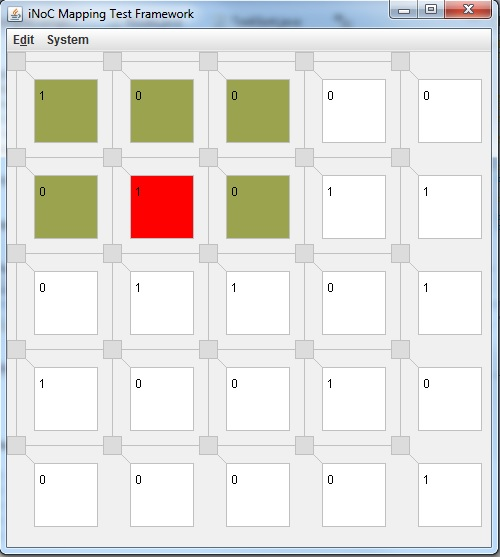
\includegraphics[width = 70mm]{bilder/NoC.jpg}
\caption{Simulation eines heterogenes Network-On-Chip: Die belegten Kacheln sind mit grün und die defekten Kacheln mit rot markiert. In jeder Kachel steht der Ressourcentyp (im Beipsiel 0 oder 1).}\label{fig:nocbild}
\end{figure}

\begin{figure}[H]\centering
  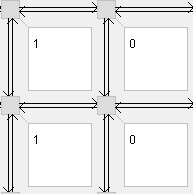
\includegraphics[width = 30mm]{bilder/Links.jpg}
  \caption{Die benachbarten Kacheln sind mit gerichteten Links in beide Richtungen verbunden.}\label{fig:links}
\end{figure}
\ \\
Jede Anwendung, die aus mehreren Teilaufgaben, den sogenannten Tasks, besteht, besitzt einen Taskgraphen (Abbildung ~\ref{fig:taskgraph}). Dieser wird zur Entwurfszeit des Programms erstellt und stellt die Anforderungen, die für eine erfolgreiche Einbettung notwendig sind, graphisch dar.

 %Die konkreten Anforderungen werden im Kapitel \todo{korrekter Verweis} näher dargelegt. \\ \\
%% die\texttt{
%%Einbettung, die für die gewünschten nicht-funktionalen Eigenschaften der Anwendung
%%während der Ausführung nötig sind. Das kann zum Beispiel ein garantierter Datendurchsatz
%%oder eine maximale Latenz sein. Es wird angenommen, dass die Anwendung periodisch
%%ausgeführt wird und regelmäßig Nachrichten zwischen den Tasks versendet. Diese
%%Kommunikation der Tasks untereinander wird mit Kommunikationsknoten dargestellt.
%%Die folgende Definition ist ähnlich zum Anwendungsgraphen in, erlaubt
%%aber, an}ders als dieser, beliebige Kommunikationsstrukturen.
\begin{figure}[H]\centering
  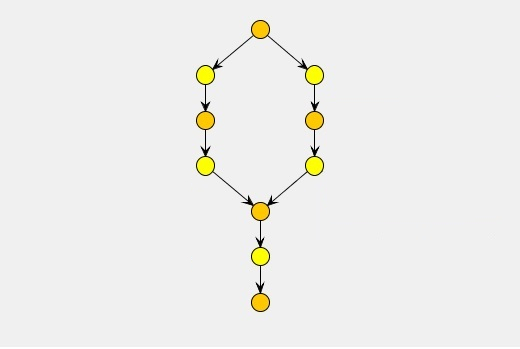
\includegraphics[width = 150mm]{bilder/taskgraph2.jpg}
  \caption{Der Taskgraph besteht aus orangefarbenen Task- und gelbgefärbten Kommunikationsknoten}\label{fig:taskgraph}
\end{figure}
\ \\
Eine Applikation besteht aus miteinander verbundenen Taskknoten $t \in T$ und Kommunikationsknoten $c \in C$. Es sind nur Kanten zwischen diesen beiden Knotentypen erlaubt. Außerdem besitzt jeder Kommunikationsknoten \textbf{genau} eine Eingangskante und eine Ausgangskante. Dem Task- und dem Kommunikationsknoten werden verschiedenartige Bedingungen übergeben, die zu erfüllen sind. Die verschiedenen Typen von Constraints sind je nach Anwendungsgebiet erweiterbar.

\begin{itemize}
\item Taskknoten $t_i\in T$
\begin{itemize}
\item \textit{TypeConstraint}: \\
Der Task benötigt einen bestimmten Kacheltyp
\item \textit{TaskWorkloadConstraint}: \\
Der Task nimmt die  Kachel zu einem gewissen Prozentsatz in Anspruch
\item \dots 
\label{Taskknoten}
\end{itemize}
\item Kommunikationsknoten $c_i \in C$:
\begin{itemize}
\item \textit{BandwidthConstraint}: \\
Jede Kommunikation benötigt jeden Link auf der Route eine bestimmte freie Bandbreite
%\item $c_i$.messageSize: Die Nachrichtengröße
%\item $c_i$.period: Das Intervall, in dem die Nachrichten geschickt werden /todo{Abstand in dem die Nachrichten geschickt werden?}
\item \textit{MaxHopConstraint}: \\
Die Route der Kommunikation darf nicht länger als eine maximale Manhatten-Distanz sein
%Maximale Manhattan-Distanz zwischen zwei Tasks, die mit einer Kommunikation in Verbindung stehen. 
\item \dots
\label{Kommunikationsknoten}
\end{itemize}

%\caption{Gesamtbild-Unterschrift}
\label{Randbedingungen}

\end{itemize}

%Hier eine Auflistung von möglichen \\ \\
%die Kanten dabei nur zwischen diesen beiden Knotentypen existieren, also nur von Task- zu
%Kommunikationsknoten und umgekehrt. Für die Kommunikationsknoten gilt zudem
%die Einschränkung, dass sie genau eine ein- und ausgehende Kante besitzen müssen. Dadurch
%sind einerseits keine Multicasts möglich und andererseits keine Kommunikation
%ohne einen Zieltask. Ein Task kann beliebig viele ein- und ausgehende Kanten haben.
%\ \\ \\
%Folgende Informationen sind im Taskgraph (Abbildung ~\ref{fig:taskgraph}) für jeden Task- bzw. Kommunikationsknoten einsehbar.
%\begin{itemize}
%\item Taskknoten $t_i\in T$
%\begin{itemize}
%\item $t_i$.ressourceRequirements: Die Anforderungen an die Ressource in Prozent
%\item $t_i$.ressourceType: Den vom Task benötigten Ressourcetypen
%\item $t_i$.ProcessingTime: Die Laufzeit des Tasks
%\label{Taskknoten}
%\end{itemize}
%\item Kommunikationsknoten $c_i \in C$:
%\begin{itemize}
%\item $c_i$.bandwidth: Die Datenübertragungsrate der Nachricht
%%\item $c_i$.messageSize: Die Nachrichtengröße
%%\item $c_i$.period: Das Intervall, in dem die Nachrichten geschickt werden /todo{Abstand in dem die Nachrichten geschickt werden?}
%\item $c_i$.hopLimit: Maximale Manhattan-Distanz (Formel ~\ref{formel2}) zwischen sendendem und empfangendem Taskknoten
%\label{Kommunikationsknoten}
%\end{itemize}
%\end{itemize}
\ \\
Das Ziel des Algorithmus ist es, für jeden Task eine Kachel zu finden, so dass alle Anforderungen des Taskgraphen erfüllt sind. Ist dies nicht möglich, soll der Algorithmus sich beenden und einen Fehlschlag der Einbettung melden. Im Abschnitt \ref{minConflicts} (Implementierung in Abschnitt \ref{minConflictImpl}) wird mit dem Min-Conflicts-Embedder ein stochastischer Ansatz vorgestellt. Es gibt auch die Möglichkeit, die Problemstellung mit dem systematischen Ansatz zu lösen. Dies wird in der Quelle \cite{jaeger} näher erläutert.

%\newpage

\section{Constraint--Satisfaction--Problem (CSP)}

Das Problem der Taskeinbettung lässt sich als Constraint-Satisfaction-Problem (CSP) formulieren. Ein CSP wird mit dem Tripel $(V, D, B)$ (Definition \ref{Def:CSP})  beschrieben. Ziel des Constraint-Satisfaction-Problems ist es, eine global konsistente Wertebelegung für alle Constraint-Variablen zu finden. Das bedeutet, es müssen alle Bedingungen erfüllt sein. Eine Bedingung ist genau dann erfüllt, wenn die Wertezuweisungen den Anforderungen der Bedingung entspricht \cite{handbuchkuenstlicheIntelligenz}. Die Bedingungen lassen sich wie in \cite{jaeger}  umformulieren. \\
\\

%\subsection{Begriffserklärung}
%Das Problem der Taskeinbettung lässt sich als Constraint-Satisfaction-Problem (CSP) formulieren. Ein CSP wird mit dem Tripel $(V, D, B)$ (Definition \ref{Def:CSP})  beschrieben. \\%(vgl. $http://www.inf.uos.de/woru/pub/diplom/html/node63.html$):
%\\
%
%%\fbox{\parbox{\linewidth}{
%
\begin{def1}[Constraint-Satisfaction-Problem \cite{artificialIntelligence}] \label{Def:CSP}
\begin{itemize}
\item V = \{$V_1$, $V_2$, \ldots , $V_n$\} ist eine endliche Menge von Variablen.
\item D = \{$D_1$, $D_2$, \ldots , $D_n$\} sind die Wertebereiche von V mit den Werten $d_i \in D_i$.
\item B = \{$B_1$, $B_2$, \ldots , $B_m$\} ist die Menge der Bedingungen, wobei jedes Randbedingung $B_j(V_j)$ eine Teilmenge $V_j = \{V_{j_1},\ldots,V_{j_m}\} \subseteq V$ der Variablen zueinander in Verbindung setzt und deren gültige Wertekombinationen auf eine Teilmenge von $D_{j_1} \times \cdots \times D_{j_m}$ beschränkt.
\end{itemize}
\end{def1}
%\ \\
%Ziel des Constraint-Satisfaction-Problems ist es, eine global konsistente Wertebelegung für alle Constraint-Variablen zu finden. Das bedeutet, es müssen alle Bedingungen erfüllt sein. Eine Bedingung ist genau dann erfüllt (Definition \ref{Def:CSPErfuellung}), wenn die Wertezuweisungen den Anforderungen der Bedingung entspricht \cite{handbuchkuenstlicheIntelligenz}:
%\\ \\
%
%\begin{def1} [Constraint-Erfüllung \cite{handbuchkuenstlicheIntelligenz}] \label{Def:CSPErfuellung}
%Gegeben sei ein CSP mit den Constraints $B_1,\ldots,B_m$ auf den Variablen $V_1, \ldots ,V_n$ mit den Wertebereichen $D_1, \ldots ,D_n$. Ein Tupel $(d_1,\ldots,d_n) \in D_1 \times \cdots \times D_n$ erfüllt ein Constraint $B_j$, $j \in \{1,\ldots,m\}$, falls die zu den Variablen von $B_j$ gehörenden Werte aus $(d_1,\ldots,d_n)$ ein Element der Relation (als entscheidbare Relation über den Variablen) von $B_j$ bilden.
%\end{def1}
%\ \\
%Eine Zuweisung $\{v_1 = d_1, v_2 = d_2, \ldots , v_k = d_k\}$ ist eine Belegung für eine Teilmenge der Variablen. Sie heißt konsistent, wenn keine der Bedingungen, für die alle relevanten Variablen zugewiesen sind, verletzt ist. Eine Lösung ist gefunden (Definition \ref{Def:LsgCSP}), wenn jeder Variablen ein Wert aus ihrem Wertebereich zugewiesen ist und sie konsistent ist. Es reicht also nicht aus, wenn jede Bedingung für sich genommen gültige Wertekombinationen aufweist. Es muss eine eindeutige Belegung der Variablen mit genau einem Wert aus dem jeweiligen Wertebereich gefunden werden, so dass alle Bedingungen erfüllt sind.\\
%
%\begin{def1}  [Lösung eines CSP \cite{handbuchkuenstlicheIntelligenz}] \label{Def:LsgCSP}
%Gegeben sei ein CSP mit den Constraints $B_1,\ldots,B_m$ auf den Variablen $V_1,\ldots,V_n$ mit den Wertebereichen $D_1, \ldots ,D_n$. Eine Lösung des CSP ist ein Tupel $(d_1,\ldots,d_n){}\in{}D_1{}\times{}\cdots{}\times{}D_n$, das $B_1, \ldots ,B_m$ erfüllt.
%\end{def1}
%\ \\
%Das Auflösen eines CSP ist somit eine Suche im Lösungsraum, welcher durch alle möglichen Lösungen aufgespannt wird. %Eine Variable kann Werte aus ihrer Domäne annehmen.
%
%
%\subsection{Anwendung des CSPs auf das Problem}\label{Randbedingungen}
%
%Für jeden Task $t_i$ wird eine Variable $V_i$ mit dem Wertebereich $D_i \subseteq K$ (siehe Abschnitt ~\ref{kacheln}) erzeugt. Der Wert $d_i \in D_i$ der Variablen ist somit eine Kachel, auf der der Task ausgeführt werden soll. $\forall$ $V_i$ $\in$ $V$ müssen folgende Randbedingungen $b_i \in B$ gelten, das heißt sie müssen als wahr (engl. \textit{True}) ausgewertet werden, um eine Lösung des CSPs zu sein:
%
%%\begin{equation}
%%\forall V_i \in V : b_res (v_i) = d_m (k_1(x_1,y_1),k_2(x_2,y_2)) = \mid x_1 - x_2 \mid + \mid y_1 - y_2 \mid 
%%\label{formel3}
%%\end{equation}
%
%\begin{itemize}
%\item Der Ressourcentyp der gewählten Kachel $d_i$  muss dem vom Task $t_i$ angeforderten Ressourcentyp entsprechen.
%
%\begin{equation}
%\forall V_i \in V:  b_{ressource}(V_i) = 
%\begin{cases}
%True,\: & wenn \ t_i.ressource = d_i.ressource\\
%False, & sonst
%\end{cases}
%\end{equation}
%
%
%\item Eine Kachel darf nur verwendet werden, falls sie nicht fehlerbehaftet ist.
%\begin{equation}
%\forall V_i \in V: b_{isOK}(V_i) = 
%\begin{cases}
%True,\: & wenn \ d_i.$istFehlerhaft $ = False \\
%False, & sonst 
%\end{cases}
%\end{equation}
%
%\item Eine Kachel muss ausreichend viel Kapazität besitzen. Ist dies der Fall, wird der Task eingebettet und die Kapazität angepasst. \\($d_i$.freeCapacity := $d_i$.freeCapacity -- $t_i$.ressourceRequirement).
%\begin{equation}
%\forall V_i \in V: b_{capacity}(V_i) =
%\begin{cases}
%True,\: & wenn \ d_i.$freeCapacity$ \geq t_i.resourceRequirement\\
%False, & sonst
%\end{cases}
%\end{equation}
%
%
%\item Die Kachel darf nur verwendet werden, wenn die Distanz zwischen zwei durch eine Kommunikation  $\forall c_i \in C$ in Verbindung stehenden eingebetteten Tasks $t_i$ und $t_j$ nicht größer als die maximale Distanz  ($c_i$.hopLimit) ist. Task $t_i$ sei hier der \emph{Sender} der Kommunikation und Task $t_j$ der \emph{Empfänger}. Der Abstand wird mit der Manhattan-Distanz (Formel \ref{formel2}) berechnet.
%\begin{equation}
%V_i,V_j \in V: b_{distance}(V_i,V_j) =
%\begin{cases}
%True, & wenn \  d_m(t_i,t_j) \leq k_i.$hopLimit$ \\
%False, & sonst 
%\end{cases}
%\end{equation}
%
%\item Jeder Link $l_j \in L$ hat nur eine gewisse Kapazität für die Nachrichtenübertragung zur Verfügung. Um die maximale Auslastung nicht zu überschreiten, werden alle Kommunikationen $c_k \in CommOnLink(l_j)$, die auf einen Link $l_j \in L$ transportiert werden, überprüft. Wenn die Summe der Bandbreite der Kommunikationen $c_k.bandwidth$ die Kapazität $ l_j.capacity$ nicht überschreitet, dann ist die Rahmenbedingung erfüllt. Die Leitungswege werden mit dem XY-Routing \cite{routingXY} berechnet. Andere Routingverfahren sind jedoch auch einsetzbar.
%
%
%\begin{equation}
%b_{routing, i}(V_1, \dots , V_{|T|}) = 
%\begin{cases}
%True, & wenn \  \forall l_j \in L : \\
%\ & \sum _{c_k \in CommOnLink(l_j, C_1,\dots C_n)} \limits c_k.bandwidth \leq l_j.capacity \\
%\ & \\
%False, & sonst
%\end{cases}
%%t_i \in T: c_{routing}(t_i) = isRoutingPossible(V_i) 
%%l_i \in L: b_{routing}(l_i) = 
%%\begin{cases}
%%True, & wenn  \sum_{c_j \in CommOnLink(l_i)} \limits c_j.bandwidth \leq l_i.capacity \\
%%False, & sonst 
%%\end{cases}
%\end{equation}
%
%\end{itemize}
%\ \\
%Die Randbedingungen $b_{ressource}$ und $b_{isOK}$ sind unäre Randbedingungen. Das heißt die Bedingungen sind abhängig von der Belegung einer einzigen Variablen. Sie können durch eine Anpassung der Domäne angepasst werden. $b_{distance}$ und $b_{capacity}$ sind binäre Randbedingungen. Dies sind Bedingungen, die von zwei Variablen abhängig sind. $b_{routing}$ ist eine Randbedingung höherer Ordnung und ist von der Belegung jeder einzelnen Variablen abhängig.
%

%\subsection{Vom Taskgraph zum Constraintgraph} \label{constraintgraph}
%
%Um von einem Taskgraph zu einem Constraintgraph \cite{foundationCSP} zu kommen, sind folgende Schritte nötig.
%
%\begin{itemize}
%\item Für jeden Taskknoten entsteht ein Knoten im Constraintgraph. Dieser Knoten repräsentiert die Variable des CSPs.
%\item Die Wertebereiche der Variablen sind die Kacheln $K$.
%\item Die Kanten zwischen den Knoten im Constraintgraph sind die Randbedingungen.
%\end{itemize}
%\ \\
%Die Abbildung \ref{fig:constraintgraph} zeigt die Umwandlung von einem Taskgraph zu einem Constraintgraphen. Es sind hier nur die $b_{distance}$-Bedingung eingezeichnet. Die unären Bedingungen können durch eine Anpassung an die jeweilige Domäne gelöst werden. Die $b_{routing}$-Bedingung verbindet alle Knoten miteinander. Dies lässt sich schwer visualisieren. Streng genommen verbindet die $b_{capacity}$-Bedingung jeden Knoten mit jedem Knoten. Dies wurde hier nicht berücksichtigt, da eine Variablenordnung mit dem Minimal-Bandwidth-Ordering Algorithmus (Abschnitt \ref{MBO}) immer die minimale Bandbreite von $n$ ($n$ Anzahl der Knoten) hätte. So wäre diese Variablenordnung nicht zielführend.
%
%%Die ist, glaub ich, dass dann alle Knoten immer die gleiche Bandbreite haben und somit auch alle Ordnungen, oder?
%
%\begin{figure}[H]\centering
%  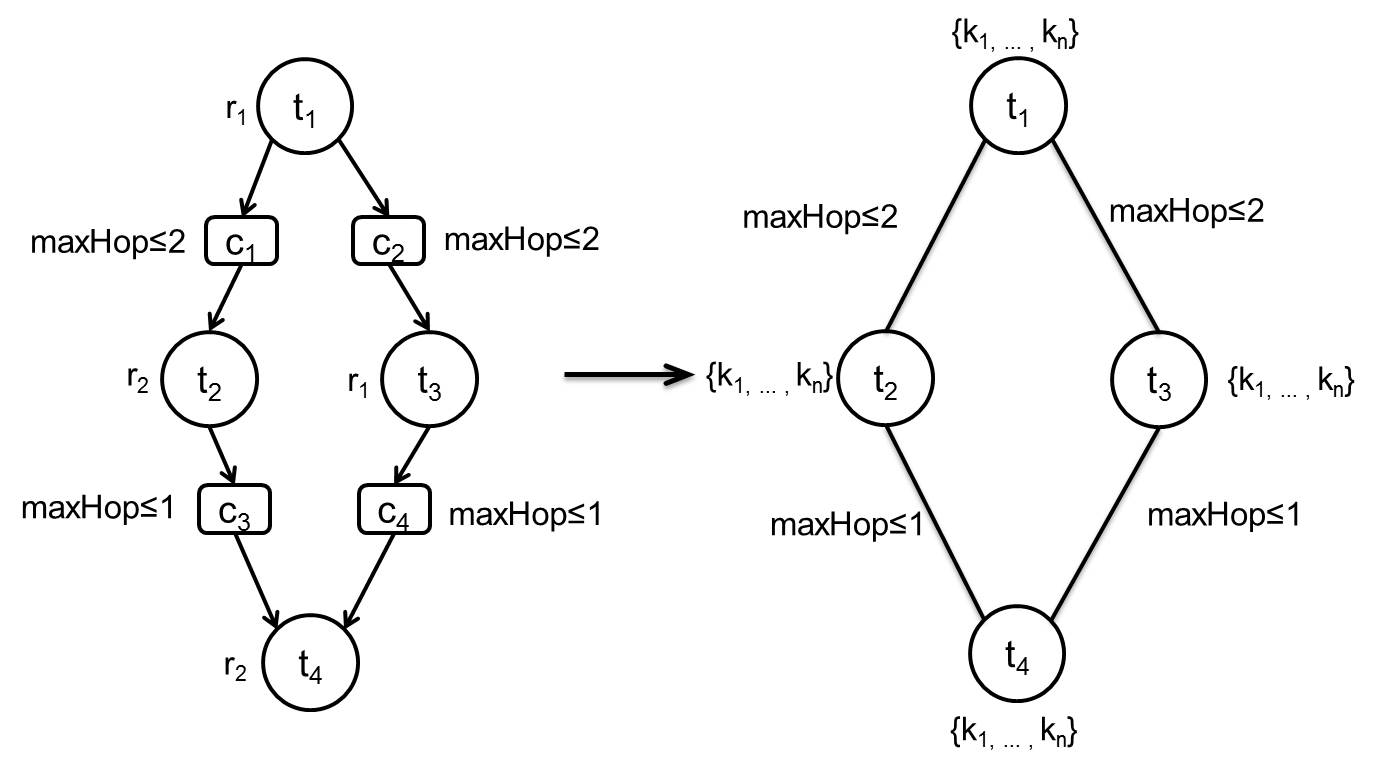
\includegraphics[width = 150mm]{bilder/taskConstraintgraph.jpg}
%  \caption{Transformation von einem Task- zu einem Constraintgraph}\label{fig:constraintgraph}
%\end{figure}

\section{Min-Conflicts-Embedder}\label{minConflicts}
Die Min--Conflicts--Heuristik ist in der Praxis eine häufig eingesetzte Methode zum Lösen von CSPs. Es handelt sich nicht um ein systematisches Verfahren wie beim Backtracking, sondern um ein Heuristisches. Als Startpunkt wird eine zufällige Belegung der Veriablen erzeugt. Falls dies keine Lösung des CSPs ist, wovon auszugehen ist, wird eine kon\-flikt\-er\-zeu\-gen\-de Variable zufällig ausgewählt. Dieser wird ein Wert zugewiesen, der möglichst wenige Randbedingungen verletzt.\\ \\
Wie bei anderen stochastischen Methoden besteht auch hier die Gefahr, dass das System in einem lokalen Minimum \todo{lokales minimum bedeutet, dass eine bestimmte Anzahl von variablen konfliktbehaftet sind und diese Anzahl ein lokales minimum darstellt? }terminiert. Das bedeutet, dass keine weiteren Verbesserungen
erzielt werden können, eine Lösung für das CSP aber noch nicht gefunden
wurde. Falls dies der Fall ist, muss eine erneute zufällige Belegung der Variablen erzeugt werden und eine neue Runde beginnt. Eine Tabu-Liste kann dabei helfen, Belegungen, die zu einem lokalen Minimum geführt haben, nicht mehr zu wählen. Nach einer vorher festgelegten Anzahl von Runden beendet sich die Heuristik und das Scheitern der Einplanung wird ausgegeben. So kann es vorkommen, dass die Min--Conflicts-Heuristik keine konsistente Lösung findet, obwohl es eine im Constraint--System gibt.\\ \\
Oftmals wird die Heuristik verwendet, wenn sich das Constraint--System geringfügig verändert hat und für das vorherige System schon eine Lösung vorhanden ist. Aus diesem Grund wird der Algorithmus auch als "heuristisches Reparieren" \cite{cspsolvingRepairMethod} bezeichnet.\\ \\

\chapter{Model zur Lösung des CSP-Problems}\label{model}

In diesem Kapitel wird zuerst die Implementierung des Min-Conflicts-Embedder (Abschnitt \ref{minConflictImpl}) mit seinen einzelnen Methoden vorgestellt. Anschließend werden anhand von Klassendiagrammen die Bindungs- (Abschnitt \ref{bindunganforderung}) und Routinganforderungen (Abschnitt \ref{routinganforderung}) näher betrachtet. Dabei wird die innere Struktur betrachtet, die diese Anforderungen hinzufügen, testen und lösen.
\section{Implementierung des Min-Conflicts-Embedder}\label{minConflictImpl}

Die Implementierung des Min-Conflicts-Embedder ist anhand des Aktivitätsdiagramm (Abbildung \ref{fig:minConflictsAkti}) graphisch dargestellt. Zuerst wird die Schleifenvariable der äußeren Schleife mit Null initialisiert und die Methode \textbf{mapTaskRandomly} aufgerufen. In \textbf{mapTaskRandomly} werden alle Tasks einer zufällig gewählten Kachel, die im Programmcode Unit genannt wird, zugewiesen. Es werden dabei Verletzungen der Constraints ignoriert. Anschließend wird der inneren Schleifenvariable k dem Wert Null zugewiesen und die Funktion \textbf{findRandomConflictingTask} aufgerufen. Diese Funktion wählt einen Task aus der Menge C der Tasks aus, die mindestens einen Constraint verletzen. Falls es keinen Task gibt (conflictingTask==null) und somit die Menge C leer ist, wurde eine Lösung gefunden (\textbf{success}). Ansonsten wird überprüft, ob die maximale Anzahl an Schleifendurchgängen (kMax) erreicht wurde. Wenn dies nicht der Fall ist, ruft das Programm die Funktion \textbf{minConflicts} auf. \textbf{minConflicts} bekommt als Parameter den conflictingTask übergeben und versucht für ihn eine geeignete Kachel zu finden, die zu keiner Verletzung eine Bindungs- bzw Routingbedingung führt. Falls es eine derartige Kachel nicht gibt, wird schrittweise der MaxHopConstraint gelockert. Das heißt, dass die Manhattendistanz schrittweise um eins erhöht wird, bis der Algorithmus eine geeignete Kachel gefunden hat. Ist dies der Fall, wird k inkrementiert und die Funktion \textbf{findRandomConflictingTask} wiederum aufgerufen. \\
Hat k den Wert kMax erreicht, so ist der Durchgang beendet und alle Tasks werden ihrer Kachel entzogen (\textbf{unmapTasks}). Die Funktion \textbf{mapTaskRandomly} wird aufgerufen und ein neuer Durchgang beginnt. Falls nach jMax Durchgängen noch keine Lösung gefunden wurde, beendet sich das Programm (\textbf{fail}).

\begin{figure}[H]\centering
  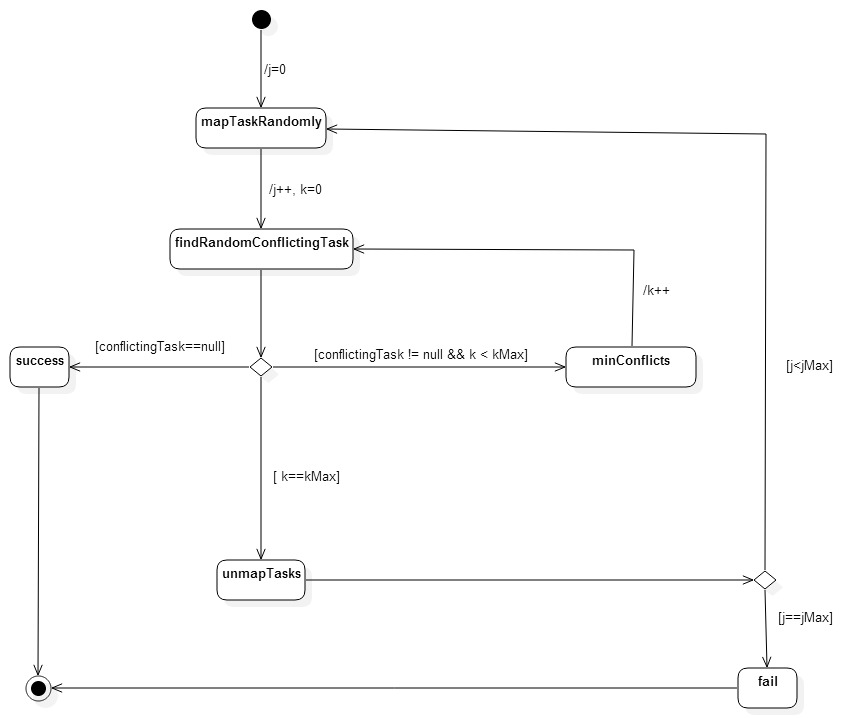
\includegraphics[width = 150mm]{bilder/minAkti.jpg}
  \caption{Das Aktivitätsdiagramm zur Min-Conflicts-Implementierung}\label{fig:minConflictsAkti}
\end{figure}
\section{Klassendiagramm zum Lösen der Bindungs- und Routinganforderungen}


\subsection{Bindungsanforderungen}\label{bindunganforderung}

Die Abbildung \ref{fig:klBind} zeigt das Klassendiagramm zum Lösen von Bindungsanforderungen. Die Klasse Task speichert in einer Liste alle Bindungsanforderungen (engl. TaskConstraint) ab und stellt folgende Funktionen zur Verfügung:

\begin{itemize}
\item \textit{addTaskConstraint}\\
fügt ein Objekt einer abgeleiteten Klasse von TaskConstraintsder Liste hinzu. 
\item \textit{removeTaskConstraint}\\
löscht ein Objekt einer abgeleiteten Klasse von TaskConstraint aus der Liste
\item \textit{taskConstraintsAreSatisfied}\\
ruft für alle Objekte in der Liste die Funktion isSatisfied aus der Klasse TaskConstraint auf. isSatisfied überprüft, ob die jeweilige Bindungsanforderung erfüllt ist. Die Funktion gibt True zurück, wenn alle Bindungsanforderungen erfüllt sind.%Es wird True zurückgegeben, wenn für alle Objektaufrufe
\item \textit{numberOfFailingConstraint}\\
gibt die Anzahl der fehlgeschlagenen Bindungsanforderungen zurück, wenn man dem Task eine Unit u zuweist. 
\item \textit{mapConstraints}\\
weist dem Task eine Unit zu. Alle Objekte, die sich in der Liste befinden, rufen die Methode map auf.
\item \textit{unmapConstraints}\\
entzieht dem Task die Unit. Alle Objekte, die sich in der Liste befinden, rufen die Methode unmap auf.
\end{itemize}

Um von der abstrakten Klasse TaskConstraints zu erben, müssen diese abstrakten Methoden implementiert werden:\\
\begin{itemize}
\item i\textit{sFeasible}\\
überprüft, ob die Anforderung erfüllt wäre, wenn der Task auf der Unit eingebettet ist. Hierzu wird die Methode \textit{check} mit der Objektvariable der zugehörigen Instanz der Klasse UnitAttribute aufgerufen.
\item \textit{sSatisfied}\\
überprüft, ob der eingebettete Task die Anforderung erfüllt. Dazu wird die Methode \textit{check} der zugerhöirigen UnitAttribute-Klasse mit dem Übergabewert null aufgerufen. 
\item \textit{map} \\
ruft von der zugehörigen UnitAttribute Unterklasse die Methode update auf. Der Parameterwert ist die eigene Objektvariable
\item \textit{}unmap\\
ruft von der zugehörigen UnitAttribute Unterklasse die Methode update auf. Der Parameterwert ist der negierte Wert der eigenen Objektvariable
\end{itemize}

Die Klasse Unit repräsentiert eine Kachel dem Network-on-Chip. Jede Instanz ist durch die Positionsangabe (x,y) eindeutig identifizierbar. Eine Instanz erhält Objekte der abgeleiteten Unterklassen von der abstrakten Klasse UnitAttributes. Die Klasse Unit befinden sich folgende Methoden:
\begin{itemize}
\item \textit{addUnitAttriubte}\\
fügt der Liste eine Objekt einer Unterklasse von UnitAttribute hinzu
\item \textit{removeUnitAttriubte}\\
löscht ein Objekt einer Unterklasse von UnitAttribute aus der Liste
\end{itemize}

Die Kindklassen von UnitAttribute müssen die zwei abstrakten Methoden \textit{check} und \textit{update} implementieren. Jede Kindklasse von TaskConstraint wird dabei von genau einer Kindklasse von UnitAttribute verwendet und überprüft ( \textit{check} ) oder aktualisiert (\textit{update} ) diese.

\begin{itemize}
\item \textit{check}\\
überprüft, ob es möglich ist, dass Attribut zu aktualisieren.
\item \textit{update} \\
aktualisiert die Objektvariable des Attributs.
\end{itemize}

%\todo{TyeAttribute wird nichts upgedated}

TypeAttribute ist ein Spezialfall. Hier kann die Objektvariable nicht, wie z. B. bei UnitWorkloadAttribute, aktualisiert werden, da sich der Ressourcentyp  nicht während der Laufzeit verändert. Deshalb ruft die Funktion \textit{update} die Funktion \textit{check} auf und überprüft, ob der gewünschte Ressourcentyp vorliegt.


\begin{figure}[H]\centering
  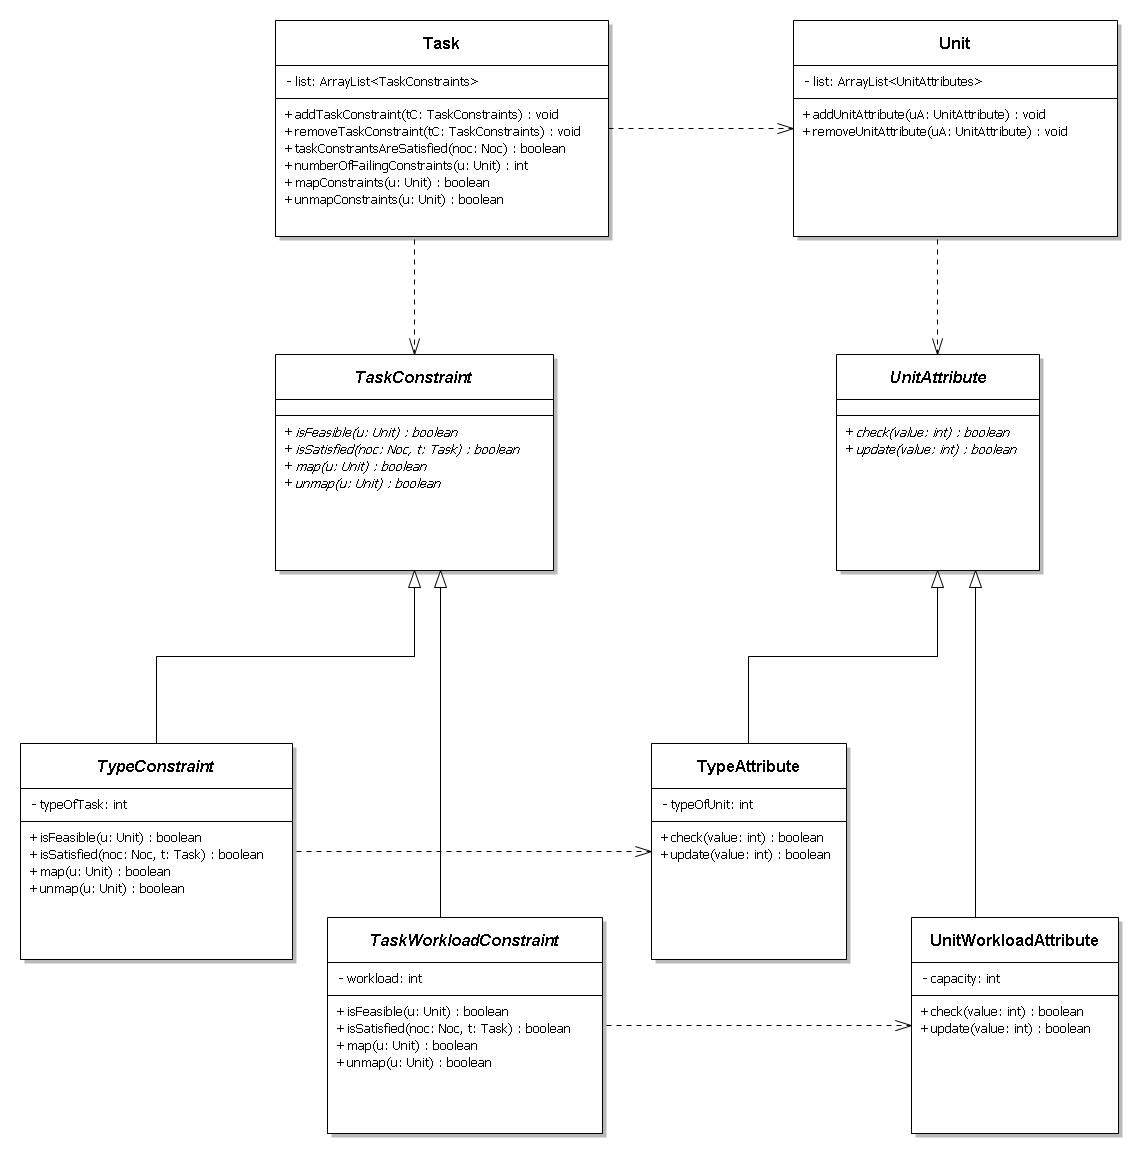
\includegraphics[width = 150mm]{bilder/task-unit.jpg}
  \caption{Klassendiagramm zum Lösen von Bindungsanforderungen}\label{fig:klBind}
\end{figure}

\subsection{Routinganforderungen}\label{routinganforderung}

Das Klassendiagramm zum Lösen von Routinganforderungen (siehe Abbildung \ref{fig:klRoute}) ist dem von Bindungsanforderungen sehr ähnlich. So sind die Methoden und deren Funktionalitäten gleich. Der Unterschied zu den Bindungsanforderungen besteht darin, dass nicht wie bei den Bindungsanforderungen die Attribute von nur einer Kachel (Unit) überprüft bzw. aktualisiert werden. Bei den Routinganforderungen werden die Attribute von mehreren Links, die zuvor mithilfe eines Routingalgorithmuses ermittelt  wurden, nachgeprüft oder erneuert. \\
\\
Die Routinganforderung MaxHopConstraint ist ein Spezialfall. Diese Anforderung benötigt kein LinkAttribut wie z. B. BandwidthConstraint, da sie nur überprüft, ob die Anzahl der Links in der zuvor berechneten Route eine maximal Zahl (maxHops) nicht überschritten wird.
\begin{figure}[H]\centering
  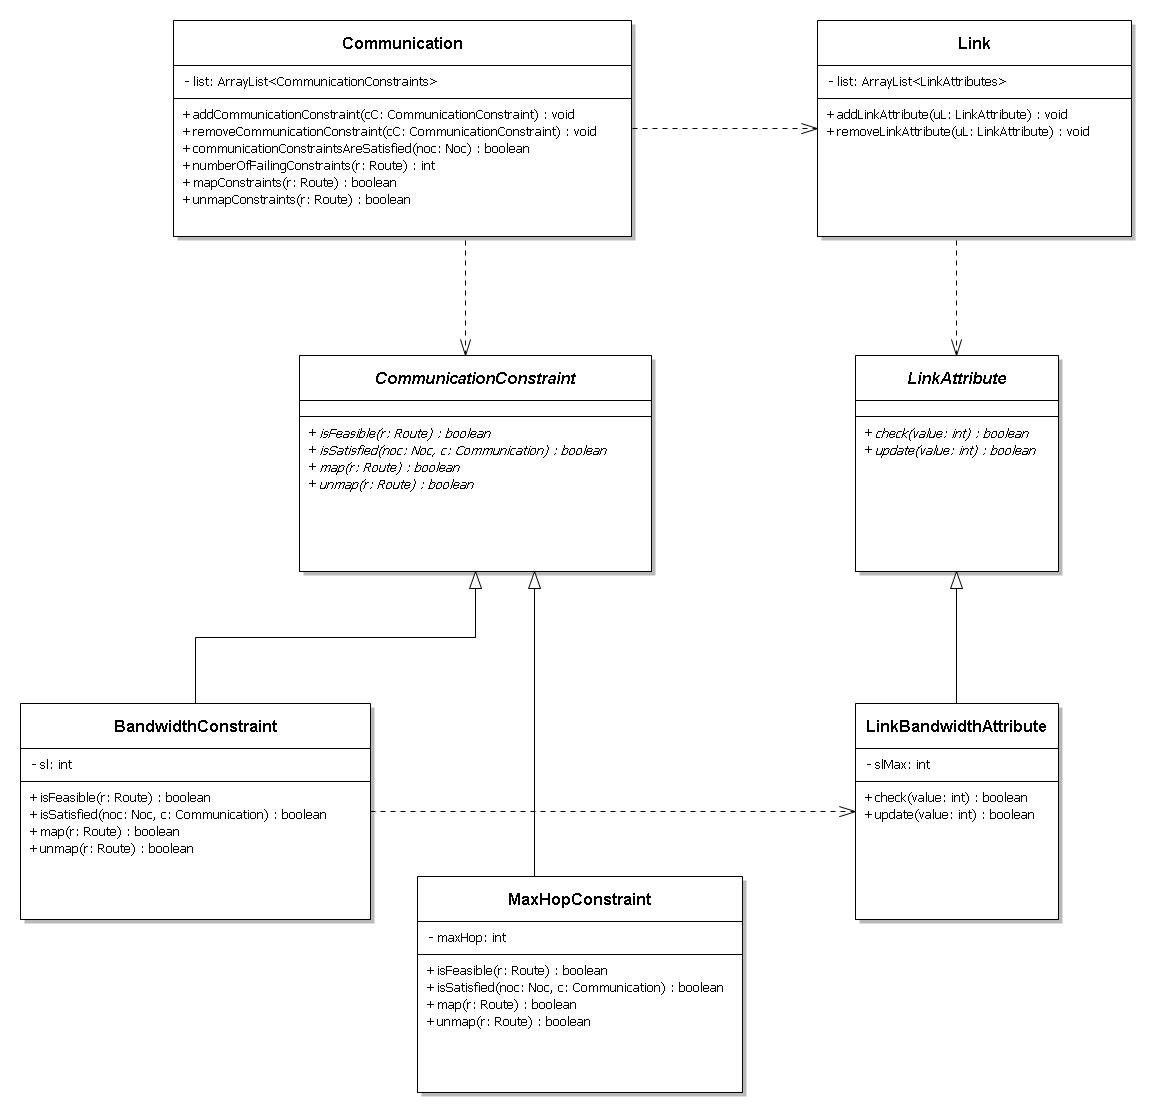
\includegraphics[width = 150mm]{bilder/communication-link.jpg}
  \caption{Klassendiagramm zum Lösen von Routinganforderungen}\label{fig:klRoute}
\end{figure}

\subsection{Hinzufügen von Anforderungen}
Um Anforderungen hinzuzufügen, wird in der Klasse Task bzw. Communication die Funktion addTaskConstraint bzw. addCommunicationConstraint aufgerufen. Die Anforderung wir in der ArrayListe list gespeichert. Falls eine Anforderung vom gleiche Typ schon vorhanden ist, wird diese durch die neue Anforderung ersetzt. Jede Anforderung (außer der MaxHopsConstraint) benötigt ein Unit- oder LinkAttribute, die beim Konfigurieren des NoCs schon mit addUnitAttribute bzw. addLinkAttribute hinzugefügt werden müssen.

\subsection{Überprüfen von Anforderungen}
Um zu überprüfen, ob alle Bindungsanforderungen erfüllt sind, wird in der Klasse Task die Methode taskConstraintsAreSatisfied aufgerufen. Diese Funktion ruft bei jedem Listeneintrag die Funktion isSatisfied. isSatisfied überprüft, ob der Task schon auf eine Kachel des Network-on-Chips eingebettet wurde und ob das dazugehörige UnitAttribute einen Fehler meldet.\\
\\
Mit der Funktion numberOfFailingConstraints in der Klasse Task kann man herausfinden, wie viele Bindungsanforderungen missachtet werden, wenn der Task zu einer Kachel zugeordnet wird. Hierzu wird für jeden Listeneintrag die isFeasible-Methode aufgerufen.\\
\\
Die Überprüfung der Routinganforderungen funktionieren nach dem gleichen Schemata.

\subsection{Zuordnen  von Anforderungen}
Wenn man die Funktion mapConstraints in der Klasse Task aufruft, werden alle für alle Listenelemente die Funktion map aufgerufen. Diese rufen, die Funktion update mit dem Übergabewert der Objektvariable des Listenelements vom dazugehörigen Attribut auf. Dadurch wird die Objektvariable des Attributs aktualisiert.\\
\\
Wenn man wieder die Anforderungen entziehen möchte, ruft man unmapConstraints auf. In dieser Funktion rufen alle Listenelemente unmap auf. Unmap ruft die Funktion update  des dazugehörigen Attriubtes auf. Diesmal ist der Übergabewert die negierte Objektvariable des Listenelements.
\chapter{Evaluierung}\label{evaluierung}

\section{Implementierung} \label{Tests}
Die Implementierung des Min-Conflicts-Embedders und der Automatismus zum Lösen von Bindungs- und Routinganforderungen wurden in der Programmiersprache X10 \cite{x10} geschrieben. Des Weiteren wurde das vom Lehrstuhl \grqq Hardware-Software-Co-Design\grqq (Universität Erlangen-Nürnberg) entwickelte CoNoC-Framework in diese parallele, objektorientierte Programmiersprache transformiert und angepasst. Für die Testumgebung wurden zwei Arten von Taskgraphen erstellt und diese mithilfe des Simulators \textit{invadeSIM} \cite{invadeSIM}  ausgewertet.

%Die Implementierung des CSP-Solver (Backtracking-Algorithmus [\ref{Backtracking}] und Min-Conflicts-Algorithmus [\ref{minConflicts}]) und der Variablenheuristiken (MWO [\ref{MWO}], MBO [\ref{MBO}], MaxHops [\ref{MaxHops}]) erfolgte in der Programmiersprache Java. Für die Simulation eines Network-On-Chips (NoC) wurde das vom Lehrstuhl \grqq Hardware-Software-Co-Design\grqq (Universität Erlangen-Nürnberg) entwickelte CoNoC-Framework verwendet. Die Taskgraphen wurden mit Hilfe des Programms \textit{Task Graphs for Free} \cite{tgff} erstellt.  \\
%\\




\section{Testumgebung} \label{Testumgebung1} 
Die Testumgebung besteht aus einem NoC, der jeweils eine Breite und eine Länge von 10 Kacheln besitzt. Die \textit{Unit-} bzw. \textit{LinkAttribute} sind folgendermaßen:
\\
\begin{itemize}
\item \textit{UnitAttribute}
\begin{itemize}
\item \textit{TypeAttribute}\\
Die Hälfte aller Kacheln sind vom Ressourcentyp 0. Der Rest ist Ressourcentyp 1.
\item \textit{UnitWorkloadAttribute}\\
Die Workload einer jeden Kachel beträgt 100.

\end{itemize}
\item \textit{LinkAttribute}
\begin{itemize}
\item \textit{LinkBandwithAttribute}\\
Die maximale Bandbreite eines jeden Links beträgt 10.
\end{itemize}
\end{itemize}

Für die Randbedingungen wurden folgende Vereinfachungen getroffen:
\begin{itemize}
\item \textit{TaskConstraint}
\begin{itemize}
\item \textit{TypeConstraint}\\
Die Hälfte aller Tasks sind vom Ressourcentyp 0. Der Rest ist Ressourcentyp 1.
\item \textit{TaskWorkloadConstraint} \\
Jeder Task benötigt eine Nutzlast von 100.
\end{itemize}
\newpage
\item \textit{CommunicationConstraint}
\begin{itemize}
\item \textit{BandwidthConstraint}\\
Jede Kommunikation benötigt eine Bandbreite von 2.
\item \textit{MaxHopConstraint}\\
Die maximale Distanz zwischen zwei miteinander kommunizierenden Tasks beträgt immer 3.
\end{itemize}
\end{itemize}

Es werden zwei Arten von Taskgraphen näher untersucht. Zum einen ein sequentieller Taskgraph (Abbildung \ref{fig:seq}), bei dem jeder Task die gleiche Anzahl an Kommunikationen besitzt,  zum anderen ein paralleler Taskgraph (Abbildung \ref{fig:par}) bei dem mehrere Kommunikationen von einem Task ausgehen. Die Tasks, die die Kommunikation empfangen, können hierbei zeitgleich weiterarbeiten. Für beide Taskgrapharten werden Taskgraphen mit jeweils $n \in \{ 3, 4, 5, 6, 7, 8, 9, 10, 11\}$ Tasks erstellt.
\begin{figure}[H]\centering
  
\includegraphics[width = 120mm]{bilder/sequentiell.jpg}
  \caption{Sequentieller Taskgraph mit $n$ Tasks: Ein Kreis repräsentiert einen Task. Ein Rechteck stellt eine Kommunikation dar.
  }\label{fig:seq}
\end{figure}

\begin{figure}[H]\centering
  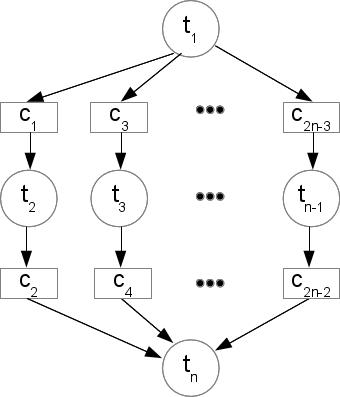
\includegraphics[width = 70mm]{bilder/parallel.jpg}
  \caption{Paralleler Taskgraph mit $n$ Tasks: Ein Kreis repräsentiert einen Task. Ein Rechteck stellt eine Kommunikation dar.}\label{fig:par}
\end{figure}

\section{Auswertung} \label{Auswertung} 

Abbildung \ref{einbettungszeit} legt dar,  wie viel Zeit der Min-Conflicts-Embedder (Abschnitt \ref{minConflicts} und \ref{minConflictImpl}) benötigt, um sequentielle bzw. parellele Taskgraphen einzuplanen. Die Taskgraphen besitzen die Eigenschaften, die im Abschnitt \ref{Testumgebung1} vorgestellt wurden. Aus der Abbildung \ref{einbettungszeit} ist deutlich zu erkennen, dass beim parallelen Taskgraph  (im Vergleich zum sequentiellen Taskgraph) mit steigender Anzahl der Tasks die benötigte Zeit sich sprunghaft erhöht. So benötigt der Embedder bei einer niedrigen Taskanzahl  für beide Taskgraphtypen etwa die gleiche Zeit, doch etwa ab zehn Tasks divergieren die beiden Graphen. Das Schaubild \ref{mips} stellt den Verlauf der benötigten MIPS (engl. \textit{Million Instructions per Second}) graphisch dar. Aus diesem Diagramm geht hervor, dass der parallele Taskgraph mehr Instruktionen pro Sekunde als der Sequentielle benötigt. Die Graphik \ref{instruktionen} stellt die Entwicklung der Gesamtzahl der Instruktionen (Formel \ref{formelInstruktionen}) dar.

\begin{equation}
Gesamtzahl der Instruktionen = MIPS * Zeit in Sekunden * 10^6
\label{formelInstruktionen}
\end{equation}

Die Schaubilder verdeutlichen, dass es sinnvoll ist, parallel einzubetten, da man bei parallelen Taskgraphen (siehe Abbildung \ref{fig:par}) $t_2$ bis $t_{n-1}$ simultan eine Lösung finden kann. Somit kann die benötigte Zeit verkürzt werden. Das Programm wurde mit der Sprache  X10 \cite{x10}  programmiert. Dies ist eine parallele, objektorientierte Programmiersprache, die speziell für high-end Hardware mit bis zu 10000 Hardware-Threads \cite{x10Spezi} , entwickelt wurde. So sollten die  kommenden Aufgaben für dieses Projekt sein, einen parallel agierende Embedder zu implementieren.
\begin{figure}
\centering
        \begin{tikzpicture}
         \pgfplotsset{every axis legend/.append style={at={(0.5,-0.18)}, anchor=north}}
                \begin{axis}[xmin=0,ymin=0,
                xlabel={Anzahl an Tasks},
                ylabel={Zeit in [ms]},
                width=1.0\textwidth,
      height=0.6\textwidth]
          %      \addplot [domain=0:80, samples=60]{1750.763223011357};
                        \addplot coordinates {
                        (0, 0)
                        (3, 29.628)
                        (4, 81.35)
                        (5, 155.8845)
                        (6, 134.531)
                        (7, 430.3)
                        (8, 505.35)
                        (9, 732.4)
                        (10, 1061.243)
                       (11, 2747.662)
};

                        \addplot coordinates {
                        (0, 0)
                         (3, 29.628)
                         (4, 43.2675)
                        (5, 151.2)
                        (6, 208.794)
                        (7, 237.3)
                        (8, 483.9455)
                        (9, 707.2)
                        (10, 601.821)
                       (11, 1313.9)
};

         \legend{paralleler Taskgraph, sequentieller Taskgraph}
                \end{axis}
        \end{tikzpicture}
\caption{Zeit, die der Embedder für die Einplanung benötigt.}
\label{einbettungszeit}
\end{figure}  





\begin{figure}
\centering
        \begin{tikzpicture}
         \pgfplotsset{every axis legend/.append style={at={(0.5,-0.18)}, anchor=north}}
                \begin{axis}[xmin=0,ymin=0,
                xlabel={Anzahl an Tasks},
                ylabel={Anzahl an Instruktionen / Zeit [MIPS]},
                width=1.0\textwidth,
      height=0.6\textwidth]
%                \addplot [domain=0:80, samples=60]{1750.763223011357};
                        \addplot coordinates {
                        (0, 0)
                        (3, 813)
                        (4, 1416)
                        (5, 1706)
                        (6, 1583)
                        (7, 1599)
                        (8, 1934)
                        (9, 1681)
                        (10, 1752)
                       (11, 1519)
};

                        \addplot coordinates {
                        (0, 0)
                         (3, 813)
                         (4, 1091)
                        (5, 1403)
                        (6, 1330)
                        (7, 1377)
                        (8, 1299)
                        (9, 1349)
                        (10, 1339)
                       (11, 1292)
};

        \legend{paralleler Taskgraph, sequentieller Taskgraph}
                \end{axis}
        \end{tikzpicture}
\caption{Anzahl der MIPS, die der Embedder benötigt.}
\label{mips}
\end{figure}  

\begin{figure}
\centering
        \begin{tikzpicture}
         \pgfplotsset{every axis legend/.append style={at={(0.5,-0.18)}, anchor=north}}
                \begin{axis}[xmin=0,ymin=0,
                xlabel={Anzahl an Tasks},
                ylabel={Anzahl an Instruktionen },
                width=1.0\textwidth,
      height=0.6\textwidth]
%                \addplot [domain=0:80, samples=60]{1750.763223011357};
                        \addplot coordinates {
                        (0, 0)
                        (3,24088)
(4,115192)
(5,265939)
(6,212963)
(7,688050)
(8,977347)
(9,1231164)
(10,1859298)
(11,4173699)


};

                        \addplot coordinates {
                        (0, 0)
                         (3,24088)
(4,47205)
(5,212134)
(6,277696)
(7,326762)
(8,628645)
(9,954013)
(10,805838)
(11,1697559)

};

        \legend{paralleler Taskgraph, sequentieller Taskgraph}
                \end{axis}
        \end{tikzpicture}
\caption{Gesamtzahl der Instruktionen, die der Embedder benötigt.}
\label{instruktionen}
\end{figure}  




%\begin{itemize}
%%\begin{tabular}{ll}
%
%\item $b_{ressource}$: \qquad $\forall t_i \in T:$ $t_i.$ressourceType $\in$ \{0,1\} \\
% 50 \% der Tasks benötigen Ressourcentyp 0  und 50 \% der Tasks Ressourcentyp 1.
%
%\item $b_{isOK}$: \qquad  $\forall k_i \in K:$ $k_i.$fehlerfrei = $True$ \\
%Alle Kacheln sind funktionsfähig.
%%\end{itemize}
%
%
%\item $b_{capacity}$: \qquad  $\forall$ $t_i \in T$: $t_i.$ressourceRequirements = 100\\
%Jeder Task benötigt die Kachel zu 100 \%. Das heißt, das auf einer Kachel nur ein Task laufen kann.
%
%
%
%\item $b_{distance}$: \qquad  $\forall t_i \in T$: $t_i$.HopLimit $\in \{1,2,3\}$\\
%Das HopLimit ist gleichverteilt zwischen 1 und 3.
%
%
%
%\item $b_{routing}$: \qquad   $\forall c_i \in C$: $c_i$.bandwidth $\cdot$ 2   =  $\forall l_j \in L$: $l_j.capacity$. \\
%Die Bandbreite jedes Kommunikationsknoten ist die Hälfte der Kapazität eines jeden Links.
%
%%\end{tabular}
%\end{itemize}
%\ \\
%Tasks können mit bis zu vier eingehenden und bis zu fünf ausgehenden Kommunikationsknoten verbunden sein.
%\ \\
%\subsection{Testumgebung 2} \label{Testumgebung2}
%Die Testumgebung 2 unterscheidet sich von Testumgebung 1 einzig bei der Rahmenbedingung $b_{routing}$.
%
%\begin{itemize}
%\item  $b_{routing}$: \qquad   $\forall c_i \in C$: $c_i$.bandwidth $\cdot$ 10   =  $\forall l_j \in L$: $l_j.capacity$. \\
%Die Bandbreite jedes Kommunikationsknoten ist ein Zehntel der Kapazität eines jeden Links.
%\end{itemize}




%Die zum Evaluieren der Algorithmen verwendeten Taskgraphen wurden mit dem Programm
%Task Graphs for Free [DRW98] generiert. Die Tasks k¨onnen mit bis zu drei
%eingehenden und zwei ausgehenden Kommunikationsknoten verbunden sein und werden
%zuf¨allig einem von drei Ressourcentypen zugeteilt. Der maximale Abstand der zugeh
%¨origen Tasks kann dabei zuf¨allig zwischen eins und neun gew¨ahlt werden.



%In diesem Kapitel soll dargelegt werden, ob Forward-Checking (Kapitel \todo{kapitel}) seine Daseinsberechtigung hat. Um dies festzustellen, wurde eine Testumgebung erstellt. Die Testumgebung besteht aus 50 verschiedenen NoCs, die jeweils eine Breite von 10 und Länge von 10 Kacheln haben. Eine Kachel ist entweder vom Ressourcentyp 0 oder den Ressourcentyp 1. Der Ressourcentyp der Kacheln wurde zufällig und gleichverteilt bestimmt. Auf den NoCs laufen zu Beginn der Einplanung keine Anwendungen. 50 \% der Tasks benötigen Ressourcentyp 0 ($t_i$.ressourceType = 0) und 50 \% der Tasks Ressourcentyp 1 ($t_i$.ressourceType = 1). Alle Kacheln sind funktionsfähig, d.h. die Nebenbedingung $b_{isOK}$ ist für jede vollständige Zuweisung erfüllt. Für die Nebenbedingung $b_{capacity}$ ist zu beachten, dass jeder Task $t_i \in T$ die Kachel zu 100 \% ($t_i.$ressourceRequirements = 100) benötigt. D.h. das auf einer Kachel nur ein Task laufen kann. Die Nebenbedingung $b_{routing}$ wurde folgendermaßen vereinfacht: $\forall c_i \in C$: $c_i$.bandwidth $\cdot$ 2   =  $\forall l_j \in L$: $l_j.capacity$. Die Bandbreite jedes Kommunikationsknoten ist die Hälfte der Kapazität eines jeden Links. Um die beiden Varianten vergleichen zu können, wurden jeweils die gleichen Taskgraphen verwendet. Jeder Taskgraph wurde auf die 50 NoCs eingeplant. Der Durchschnittswert von der Anzahl der Einplanungen für jeden Taskgraphen wurden gebildet, wobei die jeweils 15, die am meisten Einplanungsversuche, und die 15, die am wenigsten Einplanungsversuche pro Runde benötigten, verworfen wurden. Mit einer Runde ist hierbei gemeint, dass der Taskgraph auf die 50 NoCs  \\

%\section{Vergleich zwischen Backtracking mit und ohne Forward-Checking} \label{BTFC}
%
%%In diesem Kapitel soll dargelegt werden, ob Forward-Checking (Kapitel \todo{kapitel}) seine Daseinsberechtigung hat. Um dies festzustellen, wurde eine Testumgebung erstellt. Die Testumgebung besteht aus 50 verschiedenen NoCs, die jeweils eine Breite von 10 und Länge von 10 Kacheln haben. Eine Kachel ist entweder vom Ressourcentyp 0 oder den Ressourcentyp 1. Der Ressourcentyp der Kacheln wurde zufällig und gleichverteilt bestimmt. Auf den NoCs laufen zu Beginn der Einplanung keine Anwendungen. 50 \% der Tasks benötigen Ressourcentyp 0 ($t_i$.ressourceType = 0) und 50 \% der Tasks Ressourcentyp 1 ($t_i$.ressourceType = 1). Alle Kacheln sind funktionsfähig, d.h. die Nebenbedingung $b_{isOK}$ ist für jede vollständige Zuweisung erfüllt. Für die Nebenbedingung $b_{capacity}$ ist zu beachten, dass jeder Task $t_i \in T$ die Kachel zu 100 \% ($t_i.$ressourceRequirements = 100) benötigt. D.h. das auf einer Kachel nur ein Task laufen kann. Die Nebenbedingung $b_{routing}$ wurde folgendermaßen vereinfacht: $\forall c_i \in C$: $c_i$.bandwidth $\cdot$ 2   =  $\forall l_j \in L$: $l_j.capacity$. Die Bandbreite jedes Kommunikationsknoten ist die Hälfte der Kapazität eines jeden Links. Um die beiden Varianten vergleichen zu können, wurden jeweils die gleichen Taskgraphen verwendet. Jeder Taskgraph wurde auf die 50 NoCs eingeplant. Der Durchschnittswert von der Anzahl der Einplanungen für jeden Taskgraphen wurden gebildet, wobei die jeweils 15, die am meisten Einplanungsversuche, und die 15, die am wenigsten Einplanungsversuche pro Runde benötigten, verworfen wurden. Mit einer Runde ist hierbei gemeint, dass der Taskgraph auf die 50 NoCs  \\
%%\\
%
%Wie man in Abbildung \ref{fig:forwardChecking} sehen kann, benötigt man sehr viel weniger Einplanungsversuche, falls Forward-Checking (FC) zur Anwendung kommt. Wenn Forward-Checking benutzt wird, wird nur auf Kacheln einplant, die keine Randbedingung $b_i \in B$ verletzen. Vor allem die Randbedingung $b_{distance}$ verringert hierbei den Suchraum enorm. Ohne FC ist der Suchraum so groß wie  das komplette NoC. Die Maximalzahl an Einplanungen (bei 15 Tasks) betrug ohne FC 1.183.082, mit FC hingegen nur 56.385. So gab es beim Verfahren ohne FC bis zu 20 mal mehr Einplanungsversuche als mit der Verwendung von FC. Dies spiegelt in etwa das Verhältnis der Größe der Domänen in beiden Varianten wieder. %Bei der Verwendung von Backtracking ohne FC (BoFC) sind alle Kacheln in der Domäne $D_{BoFC}$ und bei der Verwendung von Backtracking mit FC (BmFC) sind nur die Kacheln  in der Domäne $D_{BmFC}$, die alle Nebenbedingungen $b_i \in B$ erfüllen, erlaubt.
%
%
%%\begin{figure}[H]\centering
%%  \includegraphics[width = 150mm]{bilder/forwardChecking.jpg}
%%  \caption{Vergleich zwischen Backtracking mit Forward--Checking und ohne Forward--Checking }\label{fig:forwardChecking}
%%\end{figure}
%
%\section{Vergleich der Variablenordnungsverfahren}
%
%In diesem Abschnitt werden die Variablenordnungsverfahren aus Kapitel \ref{variableOrdering} verglichen. Hierbei wurden die drei vorgestellten Variablenordnungsverfahren (Minimal-Bandwidth-Ordering, Minimal-Width-Ordering, MaxHops) auf die Testfälle aus Abschnitt \ref{Tests} angewandt und ausgewertet. \\
%\\
%Der Testfall 1 (Abschnitt \ref{Testumgebung1}) wurde in Abbildung \ref{fig:ordering2Links} und der Testfall 2 (Abschnitt \ref{Testumgebung2}) in Abbildung \ref{fig:ordering10Links} ausgewertet. Wie zu erwarten war, steigt der Lösungsaufwand mit der Anzahl an Tasks. Zum einen zeigt es sich, dass die schwer zu erfüllende $b_{routing}$-Bedingung aus Testfall 1 einen maßgeblichen Anteil an der Anzahl der Einplanungen auf die Kacheln besitzt. Es werden bis zu 67 mal mehr Einplanungen beim Testfall 1  als beim Testfall 2 getätigt. Zum anderen erkennt man, dass die verschiedenen Testumgebungen keinen Einfluss auf die Rangfolge der Ordnungsverfahren hat. In beiden Testumgebungen benötigt Minimal-Bandwidth-Ordering (MBO) die wenigsten Einbettungen. Mit einem eher kleinen Abstand folgt Minimal-Width-Ordering (MWO) auf Rang zwei. Sehr viel mehr Einbettungen benötigt MaxHops im Vergleich zu MBO und MWO. Deshalb ist MaxHops besonders für große Taskgraphen nicht empfehlenswert.
%
%%\begin{figure}[H]\centering
%%  \includegraphics[width = 150mm]{bilder/ordering3.jpg}
%%  \caption{Vergleich zwischen den drei vorgestellten Variablenordnungsverfahren. Testumgebung 1 stammt aus Abschnitt \ref{Testumgebung1}.}\label{fig:ordering2Links}
%%\end{figure}
%
%%\begin{figure}[H]\centering
%%  \includegraphics[width = 150mm]{bilder/variablenordnung10nachrichtenProLink.jpg}
%%  \caption{Vergleich zwischen den drei vorgestellten Variablenordnungsverfahren. Testumgebung 2 stammt aus Abschnitt \ref{Testumgebung2}.}% Die Variablenordnungen wurden in Testumgebung 2 (Abschnitt \ref{Testumgebung2}) ausgewertet. 
%%  \label{fig:ordering10Links}
%%\end{figure}
%
%%Wie man in Abbildung \ref{fig:ordering} erkennt, benötigen MWO und MBO annähernd die gleiche Anzahl an Einbettungen. Das MaxHops Verfahren fällt gegenüber den anderen zwei vorgestellten Verfahren ab. Dies liegt daran, dass MaxHops nicht nach Anzahl der Abhängigkeiten (MWO und MBO) sortiert, sondern nach der Größe der maximalen HopLimits. So ist es bei MaxHops möglich, dass ein Task der zu Beginn eingeplant werden soll, auch mit Tasks am Ende der Einplanungsordnung in Verbindung steht. \\
%%\\
%\ \\
%Obwohl MBO die wenigsten Einbettungen benötigt, ist er nicht empfehlenswert. MBO benötigt für die Berechnung der Taskreihenfolge eine Zeitkomplexität von $\mathcal O(n^k)$ ($n$ Anzahl der Tasks und $k$ minimale Bandbreite). MWO und MaxHops haben lediglich eine Zeitkomplexität  von $\mathcal O(n^2)$ ($n$ Anzahl der Tasks). Tabelle \ref{table:Zeit} und die dazugehörige Abbildung \ref{fig:Zeit} zeigen die Berechnungsdauer für die Ordnungsverfahren. Es zeigt sich, dass die Berechnungszeit für MBO zu lange dauert, um es in der Praxis anzuwenden. Deshalb ist MWO als guter Kompromiss zwischen wenigen Einplanungen und kurze Berechnungsdauer empfehlenswert.
%%Als schnellstes Ordnungsverfahren stellte sich MBO bei den Tests heraus. Der Abstand zu MWO ist nicht besonders groß. Gegen MBO spricht, dass es eine sehr hohe Zeitkomplexität von $\mathcal O(n^k)$ ($n$ Tasks und $k$ maximale Bandbreite) im Gegensatz zu MWO $\mathcal O(n^2)$ hat. Aus diesem Grund ist MWO dem MBO vorzuziehen.\\
%\\
%\begin{table}[H]\centering
%\begin{tabular} {c | c | c | c}
%\ & MWO & MBO & MaxHops \\
%\hline
%5 Tasks & 6 ms & 6 ms & 6 ms \\
%7 Tasks & 6 ms & 12 ms & 6 ms \\
%10 Tasks & 7 ms & 18 ms & 7 ms \\
%12 Tasks & 8 ms & 199 ms & 7 ms \\
%15 Tasks & 8 ms & 13.250 ms & 9 ms
%\end{tabular}
%\caption{Zeitdauer (in Millisekunden) für die Berechnung der Variablenreihenfolge.} 
%\label{table:Zeit}
%\end{table}
%
%%die Tasks im Gegensatz zu MWO und MBO nicht zwangsläufig durch Kommunikationsknoten verbunden sind. So ist es möglich, dass mehrere Tasks den 
%%\begin{figure}[H]\centering
%%  \includegraphics[width = 150mm]{bilder/ZeitmessungVariablenordnung.jpg}
%%  \caption{Zeitdauer für die Variablenordnungsverfahren}\label{fig:Zeit}
%%\end{figure}
%
%
%
%
%\section{Vergleich zwischen Min-Conflicts und Backtracking}
%
%In diesem Abschnitt wird Min-Conflicts (Abschnitt \ref{minConflicts}) mit dem Backtracking-Verfahren (Abschnitt \ref{Backtracking}) verglichen. Backtracking verwendet hierbei Forward-Checking (Abschnitt \ref{ForwardChecking}) und das Variablenordnungsverfahren Minimal-Width-Ordering (MWO, Abschnitt \ref{MWO}). Die Ergebnisse aus Testumgebung 1 (Abschnitt \ref{Testumgebung1}) werden in Abbildung \ref{fig:MinConflictTest1} und die Ergebnisse aus Testumgebung 2 (Abschnitt \ref{Testumgebung2}) werden in Abbildung \ref{fig:MinConflictsTest2} dargestellt.  \\
%\\
%Der Min-Conflicts-Algorithmus darf pro Testfall 100 Durchgänge durchlaufen. Das heißt, es können alle Tasks 100 mal neu und zufällig gesetzt werden. Pro Durchgang ist es 500 mal möglich, einen konflikterzeugenden Task auszuwählen und die Konflikte zu lösen bzw. zu minimieren. Falls es dennoch zu keiner gültigen Belegung der Tasks kommt, wird der Testfall als \textit{nicht gelöst} bewertet.\\
%\\
%Die gestrichelte Linie in beiden Abbildungen zeigt auf, mit welcher Wahrscheinlichkeit der Min-Conflicts-Embedder eine Lösung für das gegebene Problem findet. Die Wahrscheinlichkeit sinkt mit der Anzahl an Tasks. Besonders in Abbildung \ref{fig:MinConflictsTest2} sieht man deutlich, wie die Wahrscheinlichkeit, dass der Min-Conflicts-Embedder eine Lösung findet, schwindet. Die Erfolgswahrscheinlichkeit beim Backtracking-Verfahren ist jedoch immer bei 100 \%. \\
%\\
%Die durchgezogenen Linien stellen den Mittelwert der Einbettungen auf den Kacheln graphisch dar. Es werden hierbei nur erfolgreiche Einbettungsversuche gewertet.\\
%\\
%In Abbildung \ref{fig:MinConflictTest1} erkennt man, dass die Erfolgswahrscheinlichkeit für das Min-Conflicts-Verfahren deutlich sinkt. So findet der Min-Conflicts-Embedder bei der Anzahl von 15 Tasks nur in 18 \% der Fälle eine Lösung. Der Grund liegt in den schwer erfüllbaren Bedingungen der Testumgebung 1, insbesondere Bedingung $b_{routing}$. \\
%\\
%Der Verlauf der Einbettungsfunktion zeigt Folgendes: Bei einer geringen Anzahl an Tasks ist das Backtracking- und das Min-Conflicts-Verfahren annähernd gleich. Steigt die Anzahl der Tasks\footnote{das zu lösende Problem wird schwieriger}, so benötigt der Min-Conflcits-Embedder erheblich mehr Einbettungen. Der Knick an der Stelle zwischen zehn und zwölf Tasks lässt sich damit erklären, dass die Erfolgsquote von Min-Conflicts in dieser Auswertungsspanne erheblich gesunken ist. %Die NoC Noc-Architekturen ausgewertet die viele Lösungen befinden
%
%% Die wenigen erfolgreichen Einplanungsversuche verfälschen das Ergebnis, da nur die lassen keinen statistischen zu \todo{Formulierung wenige erfolgreiche Einplanungsversuche. Bei den wenigen . }
%
%%Zuerst wird die Erfolgsquote der Min-Conflicts-Heuristik (Kapitel \refminConflicts) untersucht. Hierbei werden die Testfälle aus Abschnitt \ref{Tests} wieder verwendet. Der Algorithmus darf pro Testfall 40 Durchgänge durchlaufen, das heißt es können alle Tasks 40 mal neu und zufällig gesetzt werden. Pro Durchgang ist es 200 mal möglich einen konflikterzeugenden Task auszuwählen und die Konflikte zu lösen bzw. zu minimieren. Falls es dennoch zu keiner Lösung kommt, wird der Testfall als \textit{nicht gelöst} bewertet. In Abbildung \ref{fig:MinConflictErfolgsquote} ist zu erkennen, dass es mit der ansteigender Zahl an Tasks die Min-Conflicts-Heuristik seltener eine Lösung findet, obwohl eine Lösung vorhanden ist. Das Backtracking-Verfahren findet jedoch immer eine Lösung, falls eine vorhanden ist.
%
%%\begin{figure}[H]\centering
%%  \includegraphics[width = 150mm]{bilder/MinConflicts2Links.jpg}
%%  \caption{Vergleich zwischen Backtracking mit Minimal-Width-Ordering (MWO) und Min-Conflicts. Testumgebung 1 stammt aus Abschnitt \ref{Testumgebung1}. \\
%%  Die durchgezogenen Linien geben die Einbettungen auf den Kacheln an. \\
%%  Die gestrichelte Linie gibt die Erfolgswahrscheinlichkeit der Einbettung an.}\label{fig:MinConflictTest1}
%%\end{figure}
%\ \\
%Abbildung \ref{fig:MinConflictsTest2} stellt die Auswertung der Testumgebung 2 (Abschnitt \ref{Testumgebung2}) dar. Die Erfolgsquote ist hierbei höher als bei Abbildung \ref{fig:MinConflictsTest2}. Das liegt daran, dass es mehr Lösungen auf den Network-on-Chip (NoC) gibt. Der Min-Conflicts-Embedder schneidet aber wiederum viel schlechter als der Backtracking-Embedder ab. 
%%In Abbildung \ref{fig:VergleichMinConflictBacktracking} wird das Backtracking- mit dem Min-Conflicts-Verfahren verglichen. Hierbei werden nur erfolgreiche Einbettungsversuche gewertet. Im Backtracking-Verfahren wurde Forward-Checking verwendet. Zuvor wurden die Tasks mit Hilfe dem Variablenordnungsverfahern MWO geordnet. Wie auf der Abbildung zu erkennen ist, steigt die Anzahl der Einbettungsversuche bei Backtracking stärker als bei Min-Conflicts an. Dies sieht auf den ersten Blick positiv aus. Jedoch muss die viel geringere Erfolgsquote von Min-Conflicts berücksichtigt werden. So sollte bei der gewählten Testumgebung (Abschnitt \ref{Tests}) ab einer Anzahl von 10 Tasks der Min-Conflicts als CSP-Solver nicht mehr ausgewählt werden. Min-Conflicts eignet sich vor allem als Reparaturverfahren. Wenn schon eine Lösung gefunden wurde, aber eine von einem Task benutzte Kachel defekt wird. Hier kann Min-Conflicts eine Lösung mit wenigen Einbettungsversuchen finden.
%
%%\begin{figure}[H]\centering
%%  \includegraphics[width = 150mm]{bilder/MinConflicts10Links.jpg}
%%  \caption{Vergleich zwischen Backtracking mit Minimal-Width-Ordering (MWO) und Min-Conflicts. Testumgebung 2 stammt aus Abschnitt \ref{Testumgebung2}. Die durchgezogenen Linien geben die Einbettungen auf den Kacheln an. Die gestrichelte Linie gibt die Erfolgswahrscheinlichkeit der Einbettung an.}\label{fig:MinConflictsTest2}
%%\end{figure}
%\ \\
%Die Evaluierung hat ergeben, dass das Min-Conflicts-Verfahren insbesondere für schwer zu lösende Probleme ungeeignet ist. Die Verwendung des Min-Conflicts-Verfahren für die Einbettungen einer Anwendung in einem Network-on-Chip (NoC) ist nicht zu empfehlen, falls es sich um ein schwer zu erfüllendes Problem handelt. Min-Conflicts eignet sich jedoch als Reparaturverfahren \cite{cspsolvingRepairMethod}, wenn bereits eine Lösung gefunden wurde, aber eine von einem Task benutzte Kachel defekt wird. In diesem Fall kann Min-Conflicts eine Lösung mit wenigen Einbettungsversuchen finden.

\chapter{Zusammenfassung}\label{zusammenfassung}

In dieser Projektarbeit wurde gezeigt, wie es möglich ist, Anwendungen mit Bindungs- und Routinganforderungen in einem Mehrprozessorsystem einzubetten, so dass diese leicht erweiterbar sind. Ferner wurde ein stochastischer Ansatz - der Min-Conflicts-Embedder - zum Lösen der Bindungs- und Routinganforderungen vorgestellt und dessen Implementierung dargelegt.\\
\\
Im Rahmen der Arbeit konnte anhand von Vergleichen zwischen sequentiellen und paralllelen Taskgraphen gezeigt werden, dass es zielführend ist, die Einbettungsphase auf mehreren Threads verteilt, ausführen zu lassen.Da das Programm mit der Sprache X10 programmiert wurde, die speziell für parallele Programmierung entwickelt wurde, ist der Aufwand gering, einen parallelen Embedder zu schreiben.\\
\\
Da das Programm leicht erweiterbar ist, ist es als Grundlage für die weitere Forschung im Bereich Invasive-Computing \cite{invasiveComputing} nutzbar

%In dieser Arbeit wurde das Problem der Selbsteinbettung von Taskgraphen bei Manycore-Architekturen beschrieben und in ein Constraint-Satisfaction-Problem umgewandelt. \\ 
%Weiterhin wurden das Backtracking-Verfahren (systematisches Verfahren) sowie das Min-Conflicts-Verfahren (stochastisches Verfahren) als zwei mögliche Varianten von CSP-Solvern näher erläutert und auf die Problemspezifikation angewandt. \\
%Als Mechanismus zum Löschen inkonsistenter Werte wurde Forward-Checking im Min-Conflicts-und Backtracking-Algorithmus verwendet. \\
%Variablenordnungen tragen in systematischen Verfahren dazu bei, die Anzahl der Einbettungen zu verringern. Es wurden daher drei verschiedene Arten von Variablenordnungen näher betrachtet. \\
%Abschließend wurden verschiedene Varianten anhand der Anzahl der Einbettungen miteinander verglichen. \\ 
%\\
%Im Rahmen dieser Arbeit konnte gezeigt werden, dass Forward-Checking maßgeblich dazu beiträgt, die Anzahl der Einplanungen zu verringern. 
%Es konnte festgestellt werden, dass eine Verwendung von Backtracking ohne Forward-Checking nicht sinnvoll ist.\\
%Bei den Variablenordnungen hat Minimal-Bandwidth-Ordering die geringste Zahl an Einplanungen benötigt. Die hohe Berechnungsdauer von $\mathcal O(n^k)$ macht diese Variablenordnung für die praktische Anwendung unbrauchbar, wohingegen sich Minimal-Width-Ordering als guter Kompromiss zwischen Berechnungsaufwand und Anzahl an Einplanungen gezeigt hat. Die MaxHops-Variablenordnung benötigte eine deutlich höhere Anzahl an Einplanungen.
%
%In dieser Arbeit wurden die drei genannten Variablenordnungen jeweils statisch vor der Einplanungsphase berechnet. Eine andere, in dieser Arbeit nicht untersuchte Möglichkeit ist es, die nächste Variable erst in der Einplanungsphase dynamisch zu bestimmen. Minimum-Remaining-Values (MRV) \cite{artificialIntelligence},  auch unter dem Namen Fail-First-Principle (FFP) \cite{foundationCSP} bekannt, kann dazu verwendet werden. In auf dieser Arbeit aufbauenden Untersuchungen ist zu prüfen, ob der erhöhte Rechenaufwand in der dynamischen Einplanungsphase durch eine Verringerung der Einplanung gerechtfertigt ist. 
%
%Das Min-Conflicts Verfahren hat sich aufgrund abnehmender Erfolgswahrscheinlichkeiten als unbrauchbar für die praktische Anwendung erwiesen. Das Backtracking-Verfahren, welches in diesen Untersuchungen deutlich besser abgeschnitten hat, sollte weiterentwickelt werden. So könnte der Suchraum durch das Ausnutzen von Symmetrien\cite{Symmetrie} weiter eingeschränkt werden. 
%



\appendix
\ifthenelse{\boolean{englishDocument}}{}{ \renewcommand{\bibname}{Literatur} }
\bibliographystyle{alpha}
\bibliography{literature}
%\input{qutellcode}
\cleardoublepage

\selectlanguage{german}
\chapter*{Erklärung}
\thispagestyle{empty}
Ich versichere, dass ich die Arbeit ohne fremde Hilfe und ohne Benutzung
anderer als der angegebenen Quellen angefertigt habe und dass die
Arbeit in gleicher oder \"ahnlicher Form noch keiner anderen
Pr\"ufungsbeh\"orde vorgelegen hat und von dieser als Teil einer
Pr\"ufungsleistung angenommen wurde.
Alle Ausf\"uhrungen, die w\"ortlich oder sinngem\"a\ss{}
\"ubernommen wurden, sind als solche gekennzeichnet.
\\[2cm]
Erlangen, \ifthenelse{\boolean{englishDocument}}
	{\date{\dateenglish{\today}}}
    	{\date{\dategerman{\today}}}
\\[3cm]
\rule{6cm}{0.5pt}\\
\parbox[l][1cm][c]{6cm}{\hfill \studname \hfill\vbox{}}






\end{document}